%-------------------------------------------------------------
% Auteur: Adrien Llave
% Date: novembre 2022
%
% TODO:
%	- add picture for first title frame
%	- scalar product: add animation of two vectors
%-------------------------------------------------------------
\documentclass[9pt, aspectratio=169]{beamer}
\usetheme{Darmstadt}
\usecolortheme{beaver}
\usepackage[french]{babel}
\usepackage{appendixnumberbeamer}
\usepackage{textpos}
\usepackage{xcolor}
\usepackage{caption}
\usepackage{subcaption}
\usepackage{array}
\usepackage[many]{tcolorbox} 
\usepackage{makecell}
\usepackage{setspace}

\usepackage{stackengine}
\usepackage{scalerel}

%\usepackage[UTF8]{ctex}
%\usepackage{hyperref}
\usepackage[T1]{fontenc}
%
%\usepackage{latexsym,multicol,booktabs,calligra}
\usepackage{amsmath,amssymb} 
%\usepackage{graphicx,pstricks,stackengine}      %   
	
\usepackage{graphicx}
\usepackage[export]{adjustbox}

\usepackage{animate} % to include a GIF movie

\usepackage{bibentry}
\nobibliography*


\captionsetup{labelformat=empty,labelsep=none,font=tiny, textfont=it}
\setbeamerfont{caption}{size=\tiny, shape=\itshape}
\setlength\belowcaptionskip{-2pt}
%\setbeamerfont{caption name}{series=\bfseries}
%\DeclareCaptionLabelFormat{mycaption}{\usebeamercolor[fg]{caption name}#1 #2. }
%\captionsetup[figure]{labelformat=mycaption, labelsep=none, labelfont=bf}

\beamertemplatenavigationsymbolsempty % remove navigation line
\setbeamertemplate{footline}[frame number] % add frame number

\definecolor{myred}{rgb}{0.8, 0.0, 0.0} % define red
\definecolor{csviolet}{rgb}{0.588, 0.008, 0.235} % define CS violet
\definecolor{dgreen}{rgb}{0.,0.6,0.}

\setbeamercolor{section in head/foot}{fg=csviolet}
 	
\setbeamercolor{itemize item}{fg=csviolet}
\setbeamercolor{itemize subitem}{fg=cyan}
\setbeamertemplate{itemize item}[circle]
\setbeamertemplate{itemize subitem}[triangle]

\setbeamercolor{section number projected}{bg=csviolet}
\setbeamertemplate{sections/subsections in toc}[circle]

% new env without headline
\makeatletter
    \newenvironment{withoutheadline}{
        \setbeamertemplate{headline}[default]
        \def\beamer@entrycode{\vspace*{-\headheight}}
    }{}
\makeatother

\makeatletter
    \newenvironment{withoutfootline}{
        \setbeamertemplate{footline}[default]
        \def\beamer@entrycode{\vspace*{-\headheight}}
    }{}
\makeatother

%\addtobeamertemplate{frametitle}{}{
%\begin{textblock*}{100mm}(.97\textwidth,-1cm)
%\includegraphics[height=0.4cm]{fig/logos/CentraleSupelec.png}\vspace{-0.9cm}
%\end{textblock*}}

%\setbeamertemplate{footline}{% 
%  \hfill% 
%  \usebeamercolor[fg]{page number in head/foot}% 
%  \usebeamerfont{page number in head/foot}% 
%  \insertframenumber%
%  %\,/\,\inserttotalframenumber
%  \kern1em\vskip2pt% 
%}

\definecolor{crimson}{rgb}{0.86, 0.08, 0.24}
\definecolor{myGreen}{rgb}{0.2, 0.71, 0.2}
\definecolor{babyblue}{rgb}{0.54, 0.81, 0.94}
\definecolor{tabblue}{RGB}{31, 119, 180}


\newtcolorbox{myblockred}[1]{%
    tikznode boxed title,
    enhanced,
    arc=3mm,
    interior style={white},
    attach boxed title to top center= {yshift=-\tcboxedtitleheight/2},
    fonttitle=\bfseries,
    colbacktitle=white,coltitle=crimson,
    boxed title style={size=normal,colframe=white,boxrule=0pt},
    before upper={\parindent15pt},
    title={#1}
}

\newtcolorbox{myblockgreen}[1]{%
    tikznode boxed title,
    enhanced,
    arc=3mm,
    interior style={white},
    attach boxed title to top center= {yshift=-\tcboxedtitleheight/2},
    fonttitle=\bfseries,
    colbacktitle=white,coltitle=myGreen,
    boxed title style={size=normal,colframe=white,boxrule=0pt},
    before upper={\parindent15pt},
    title={#1}
}

\newtcolorbox{myblockblue}[1]{%
    tikznode boxed title,
    enhanced,
    arc=3mm,
    interior style={white},
    attach boxed title to top center= {yshift=-\tcboxedtitleheight/2},
    fonttitle=\bfseries,
    colbacktitle=white,coltitle=babyblue,
    boxed title style={size=normal,colframe=white,boxrule=0pt},
    before upper={\parindent15pt},
    title={#1}
}


%% COMMAND
\newcommand{\dbspl}{dB$_{\text{SPL}}$}
\newcommand{\dms}{$\Delta$MS}
\newcommand{\dsnr}{$\Delta$SNR}
\newcommand{\DSNR}{\Delta \text{SNR}}
\newcommand{\vect}[1]{\boldsymbol{#1}}
\newcommand{\thc}{^\text{th}}
%
\newcommand{\wv}{\boldsymbol{w}}
\newcommand{\xv}{\boldsymbol{x}}
\newcommand{\yv}{\boldsymbol{y}}
\newcommand{\hv}{\boldsymbol{h}}
\newcommand{\nv}{\boldsymbol{n}}
\newcommand{\gv}{\boldsymbol{g}}
\newcommand{\qv}{\boldsymbol{q}}
%
\newcommand{\sv}{\boldsymbol{s}}
\newcommand{\Hm}{\boldsymbol{H}}
\newcommand{\Gm}{\boldsymbol{G}}
\newcommand{\covss}{\boldsymbol{\Phi}_{\sv}}
%
\newcommand{\covxx}{\boldsymbol{\Phi}_{\xv}}
\newcommand{\covnn}{\boldsymbol{\Phi_{\nv}}}
\newcommand{\cohnn}{\boldsymbol{\Gamma}_{\nv}}
\newcommand{\cohdiff}{\boldsymbol{\Gamma}_{\text{diff}}}
\newcommand{\snrout}{\rho_{\text{out}}}
\newcommand{\esp}[1]{\mathbb{E}\left[#1\right]}
\newcommand{\m}[1]{\mathcal{M}_#1}

\newcommand{\Le}{\text{L}}
\newcommand{\Rea}{\text{R}}

\newcommand{\kl}{{k, \ell}}
\newcommand{\kpl}{{\kappa, \ell}}
\newcommand{\argmin}[2]{\underset{#1}{\text{argmin}} \left\lbrace #2 \right\rbrace}

\newcommand{\xmark}{\textcolor{red}{\ding{55}}}

\newcommand{\mwfnl}{\text{\scalebox{0.8}{MWF-N, L}}}
\newcommand{\tildep}{{\tilde{\text{p}}}}

\newcommand\dangersign[1][2ex]{%
  \renewcommand\stacktype{L}%
  \scaleto{\stackon[1.3pt]{\color{red}$\triangle$}{\tiny\bfseries !}}{#1}%
}



\title{}
\author{Adrien Llave}
\institute{CentraleSupélec/IETR}

%—-------------------------------------------------------------
\begin{document}

\begin{withoutheadline}
\begin{withoutfootline}
\begin{frame}
	\vspace{0.5cm}
	% Title
	\textbf{\large Mixage automatique}
	
	\vspace{0.7cm}
	{\small Adrien Llave}

	\footnotesize novembre 2022
\end{frame}
\end{withoutfootline}
\end{withoutheadline}

% --- TOC ------------------------------------------------------------------
\begin{withoutheadline}
\begin{frame}{Sommaire}
	\tableofcontents[sectionstyle=show,subsectionstyle=show/shaded/hide,subsubsectionstyle=show/shaded/hide]
\end{frame}
\end{withoutheadline}


%==================================================================================================
%==================================================================================================
%==================================================================================================
\section{Contexte \& problématiques}

\begin{frame}{Les objectifs du mixage} %-----------------------------------------------------

\pause
\begin{itemize}
	\item équilibre entre les sources
	\item démasquer les sources
	\item maitriser la dynamique (court et long terme)
	\item composer une scène sonore
	\item transmettre de l'émotion / soutenir le propos de la musique
\end{itemize}
voir \cite{owsinski_mixing_2013}
\end{frame}


\begin{frame}{Disclaimer : charge de valeur (vertu)} %-----------------------------------------------------
Dans la review de \cite{de_man_ten_2017} :

\vspace{.8cm}
"Innovation has traditionally been met with resistance and scepticism, in particular from professional users who \textbf{fear} seeing their roles disrupted or made \textbf{obsolete}.
Music production technology may be especially susceptible to this kind of opposition, as it is characterised by a tendency towards \textbf{nostalgia}, skeuomorphisms and analogue workflows, and it is concerned with \textbf{aesthetic value} in addition to technical excellence and efficiency."

\begin{columns}
    \begin{column}{0.58\textwidth}
		
"These advancements have changed the nature of the sound engineering profession from primarily \textbf{technical} to increasingly \textbf{expressive}."

\vspace{.8cm}

"There is economic, technological and artistic \textbf{merit} in exploiting the immense computing power and flexibility that today’s digital technology affords, to venture away from the rigid structure of the traditional music production toolset."
    \end{column}
    \begin{column}{0.4\textwidth}
    \begin{figure}
		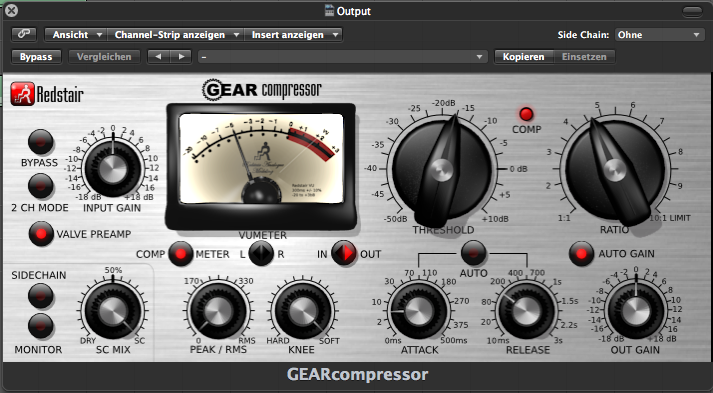
\includegraphics[width=\textwidth]{fig/Redstair_GEARcompressor.png}
		\caption{Exemple du plug-in Gear Compressor de Redstair}    
    \end{figure}
    \end{column}
\end{columns}

\end{frame}


\begin{frame}{Objectifs} %-----------------------------------------------------
\pause
\begin{itemize}
	\item Mixer des enregistrements pour des musicien.nes fauché.es
	\item Mixer de concert en bar
	\item Mixer du jeu vidéo \cite{schmidt_interactive_2003}
	\item Effectuer les tâches ingrates pour soulager les ingés son
\end{itemize}

Frontière flou entre outils d'assistance au mixage et mixage automatique total

\end{frame}


\begin{frame}{Les outils du mixage} %-----------------------------------------------------

\begin{itemize}
	\item gain
	\item panning
	\item égalisation (EQ)
	\item compression (de dynamique)
	\item correction de délai
	\item reverb
	\item distortion (compliqué !)
\end{itemize}

\end{frame}

\begin{frame}{Mixage automatique : historique de la recherche} %-----------------------------------------------------

\begin{itemize}
\item historique :
\begin{itemize}
	\item origine 2007 - 2010 : gain, pan, EQ
	\item depuis 2012 : compression
	\item depuis 2016 : arrivée de l'apprentissage profond (deep learning)
	\item depuis 2016 : reverb automatique
\end{itemize}

\item voir \cite{de_man_ten_2017} pour une revue entre 2007 et 2017

\item voir \cite{miranda_handbook_2021} pour une revue moins détaillée mais plus récente
\end{itemize}
\end{frame}

%==================================================================================================
%==================================================================================================
%==================================================================================================
\section{Effets audio et paramétrage}
\begin{frame}{Principe général} %---------------
\begin{figure}
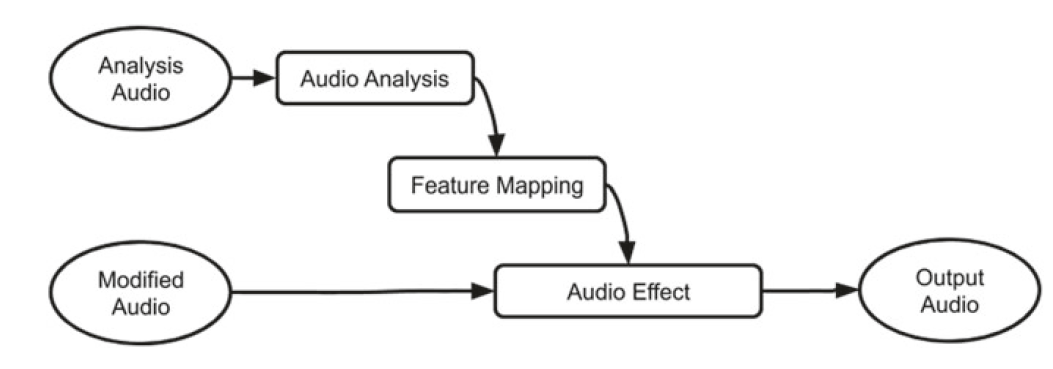
\includegraphics[width=.7\textwidth]{fig/adaptive_audio_effect_typical.png}
\end{figure}

A faire en boucle jusqu'à "convergence"

\end{frame}

\begin{frame}{Différents niveaux de complexité} %---------------
\begin{figure}
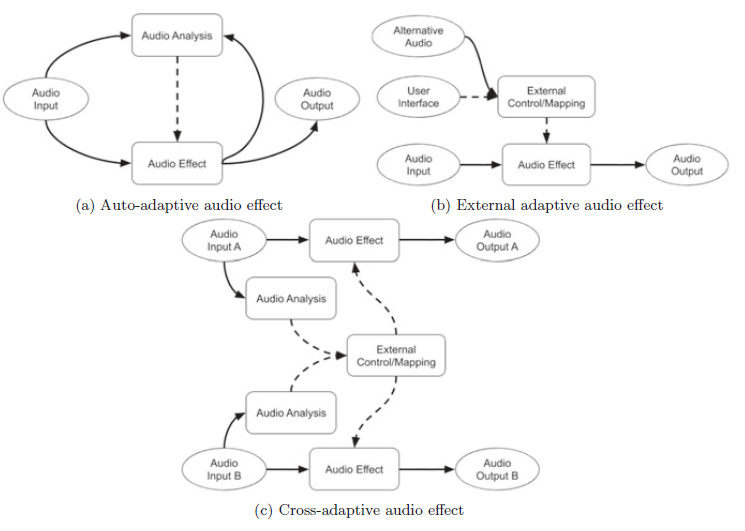
\includegraphics[width=.6\textwidth]{fig/mixauto_audiomanip.png}
\end{figure}

Revue détaillée des \emph{cross-adaptive effects} \cite{reiss_applications_2018}

\end{frame}

\begin{frame}{Traitement direct ou via effets communs ?} %---------------

\begin{itemize}
	\item Problème de l'ordre des traitements par exemple
	\item Transformation directe du signal
	\begin{itemize}
		\item plus souple (ordre des traitements)
		\item plus créative
	\end{itemize}
\end{itemize}


\begin{figure}
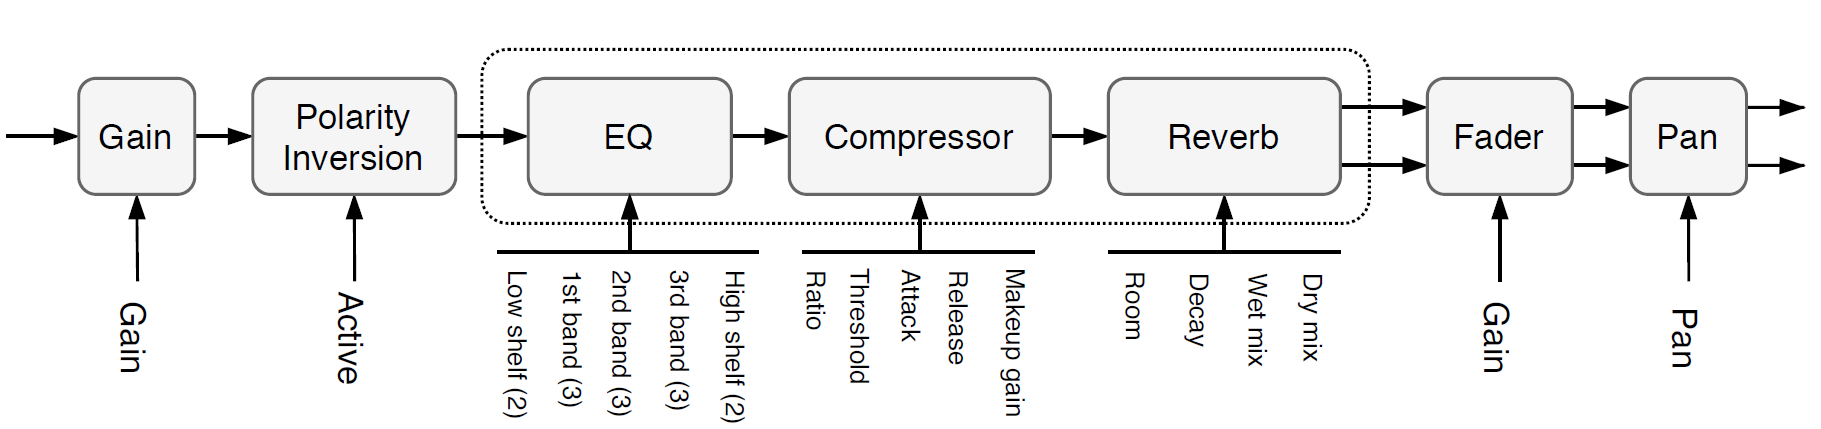
\includegraphics[width=.6\textwidth]{fig/channel_strip.png}
\caption{Chaine de traitement classique}
\end{figure}

\begin{figure}
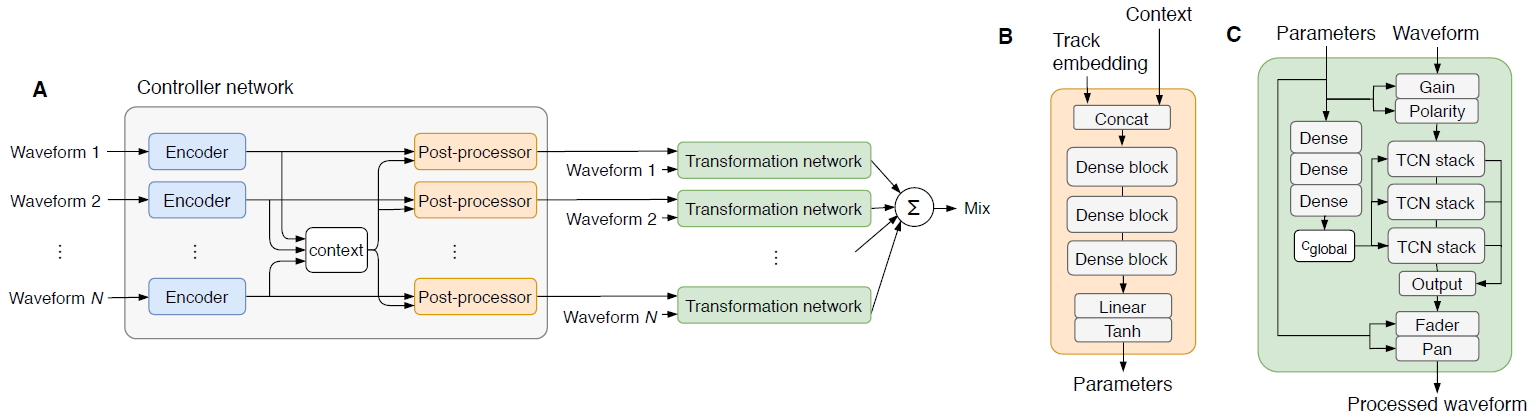
\includegraphics[width=.7\textwidth]{fig/steinmetz2021_diffmix.png}
\caption{Réseau de neurones de \cite{steinmetz_automatic_2020}}
\end{figure}
\end{frame}

\begin{frame}{Traitement direct ou via effets communs ?} %---------------
\begin{figure}
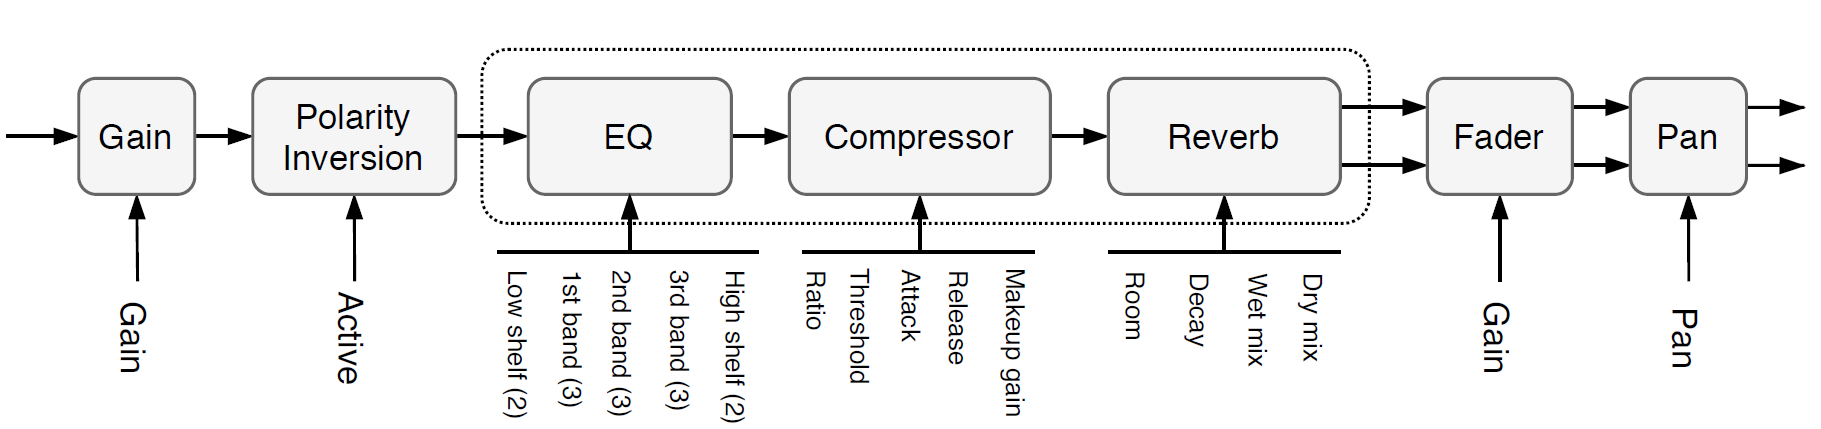
\includegraphics[width=.6\textwidth]{fig/channel_strip.png}
\caption{Chaine de traitements classique}
\end{figure}

\begin{figure}
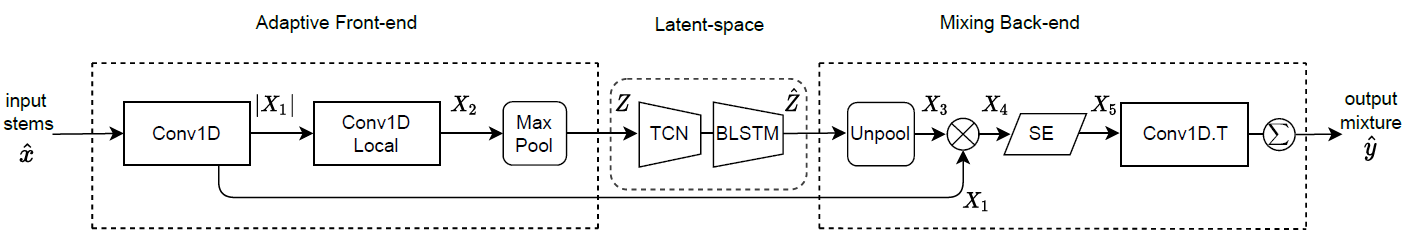
\includegraphics[width=\textwidth]{fig/martinez_ramirez2022_architecture.png}
\caption{Réseau de neurones de \cite{martinez-ramirez_automatic_2022}}
\end{figure}
\end{frame}

%==================================================================================================
%==================================================================================================
%==================================================================================================
\section{Systèmes experts}

\begin{frame}{Principe général} %-----------------------------------------------------
\begin{columns}
    \begin{column}{0.58\textwidth}
    
    \begin{itemize}
    	\item système basé sur les méthodes humaines
    	\item système basé sur des critères objectifs 
    	\item modélisation du processus de décision humain
    	\item cascade de règles \emph{si-alors-sinon}
    \end{itemize}

    \end{column}
    \begin{column}{0.4\textwidth}
		\begin{figure}
			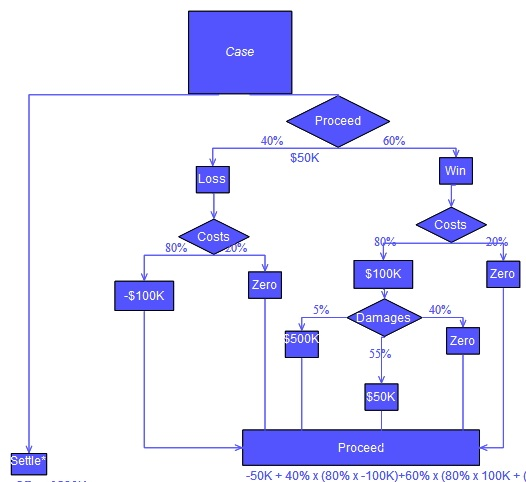
\includegraphics[width=\textwidth]{fig/decision_tree.jpg}
			\caption{Arbre de décision}
		\end{figure}
		
    \end{column}
\end{columns}
\end{frame}

\begin{frame}{Notion d'espace d'optimisation} %--------------------------
Imaginez, un espace...
\begin{figure}
\only<1>{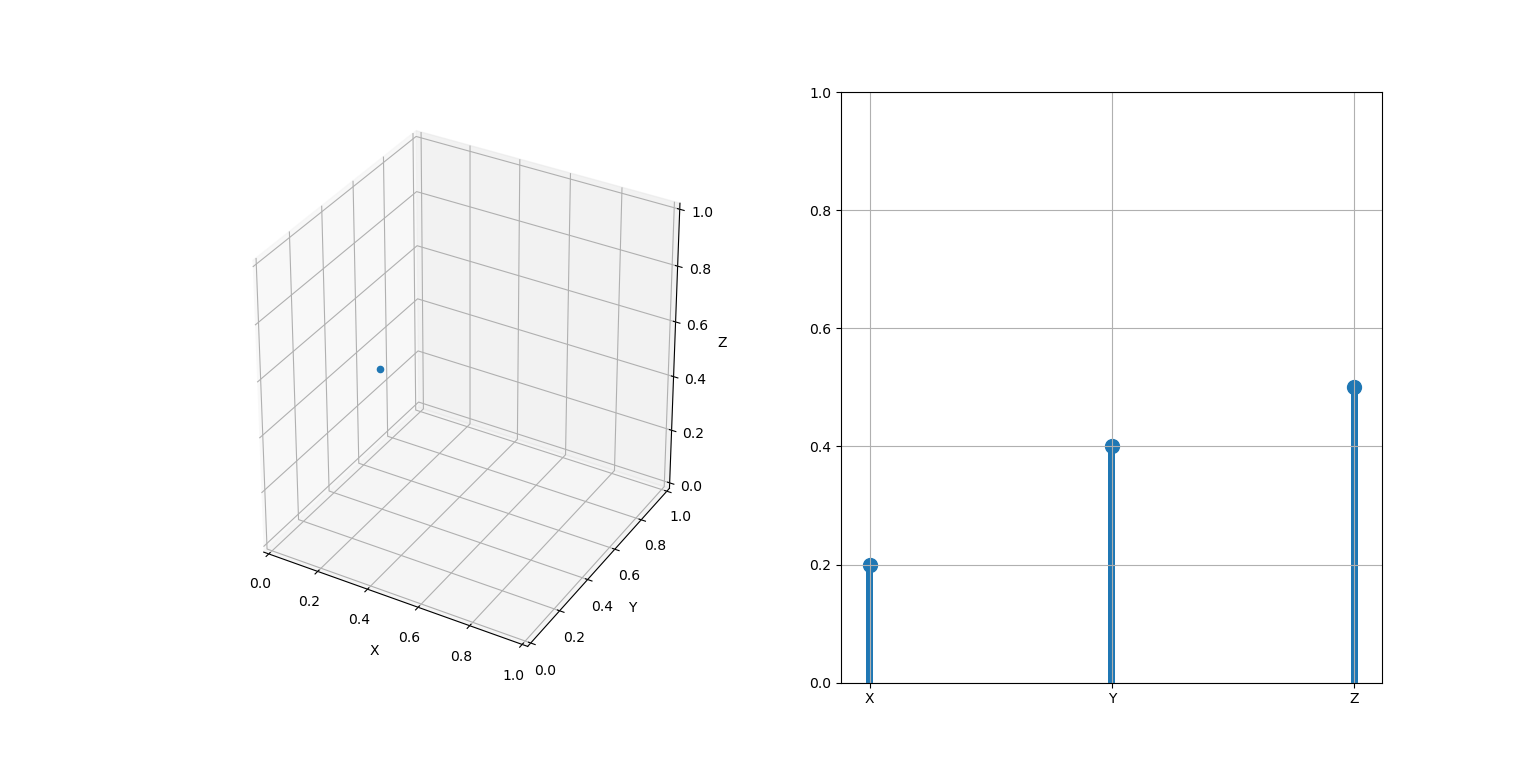
\includegraphics[width=.5\textwidth]{fig/space3d_1.png}}
\only<2>{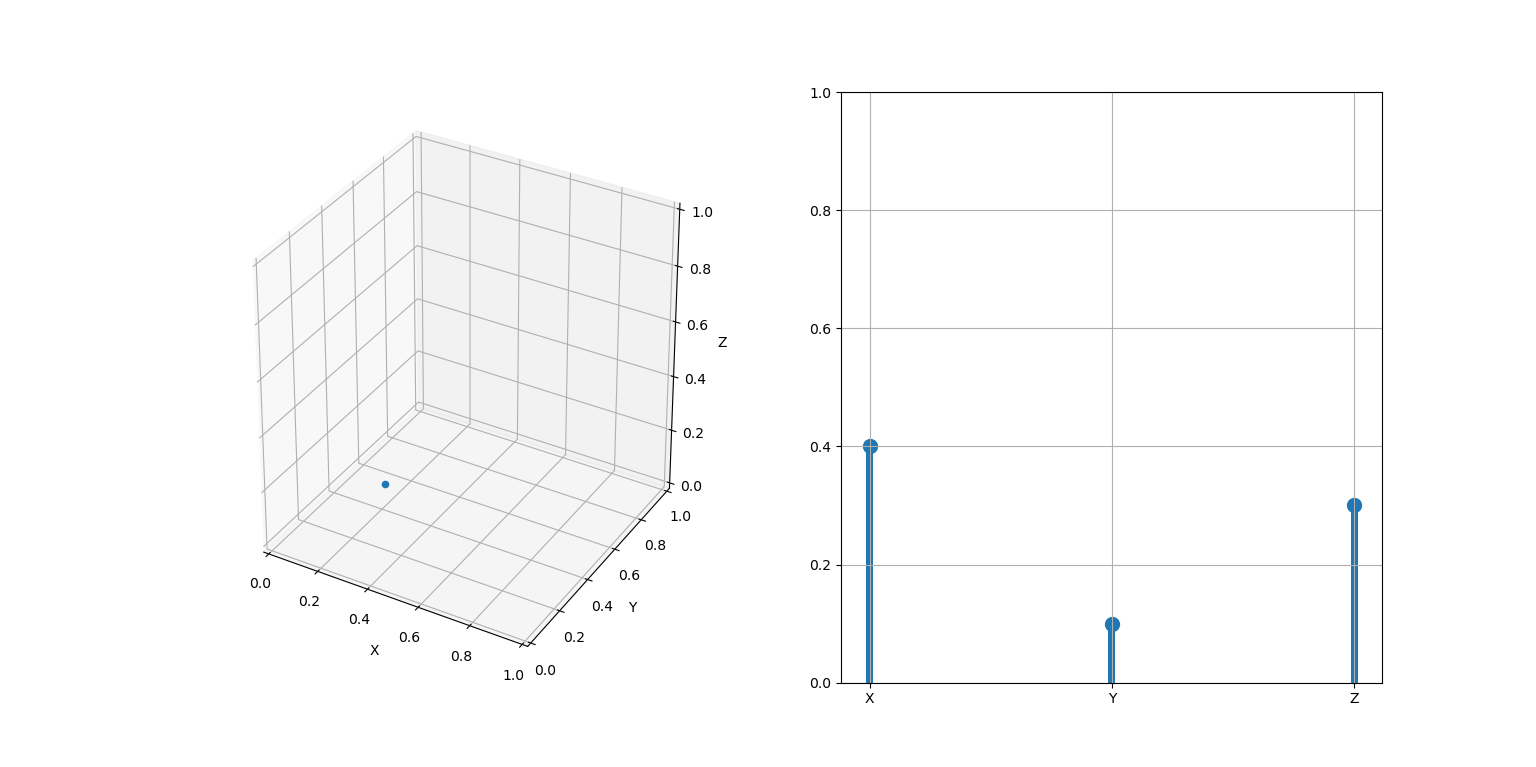
\includegraphics[width=.5\textwidth]{fig/space3d_2.png}}
\only<3->{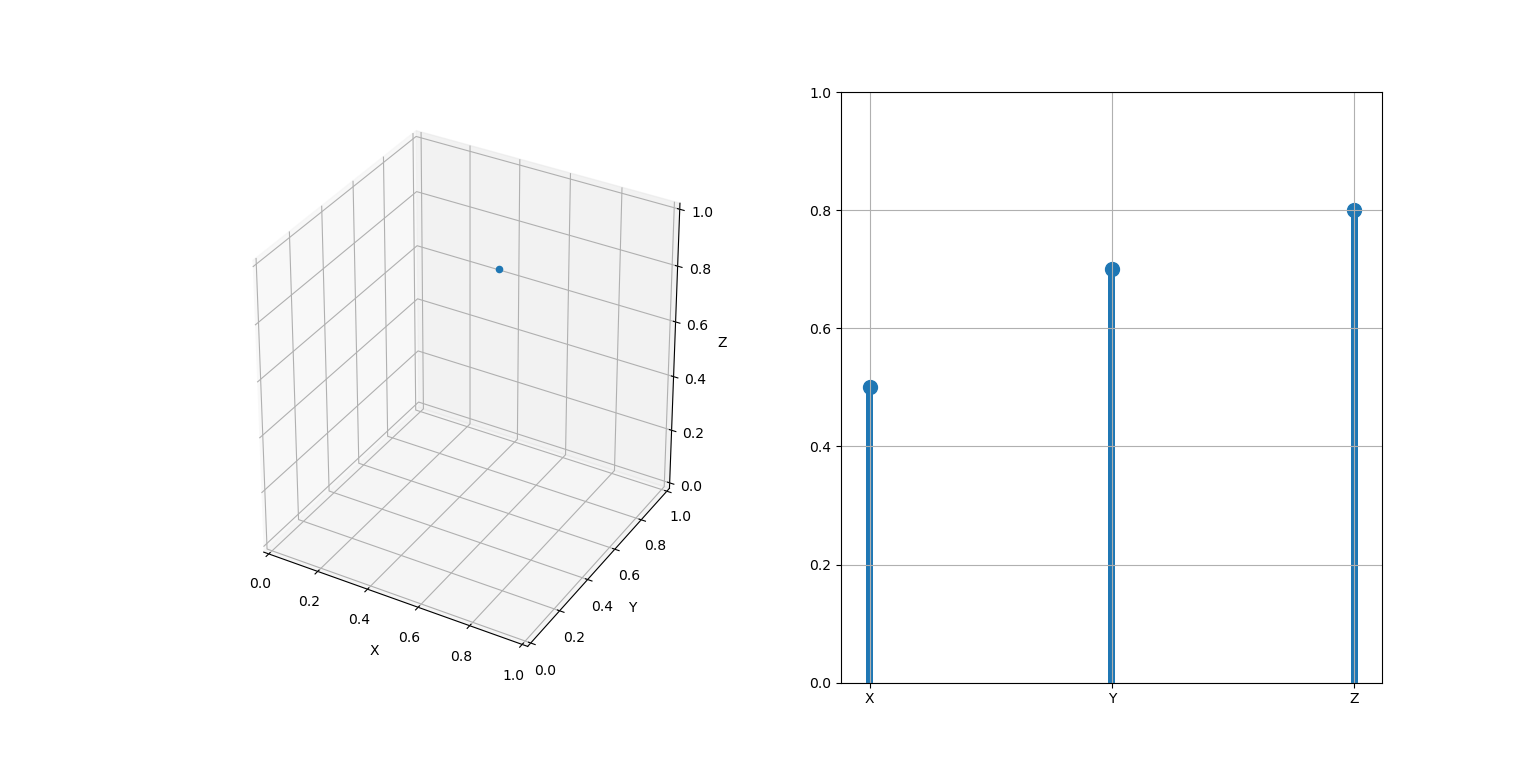
\includegraphics[width=.5\textwidth]{fig/space3d_3.png}}
\end{figure}

Un vecteur/point de l'espace = un signal

\end{frame}


\begin{frame}{Notion d'espace d'optimisation} %--------------------------
\begin{columns}
    \begin{column}{0.6\textwidth}
Imaginez, un espace à N dimensions...

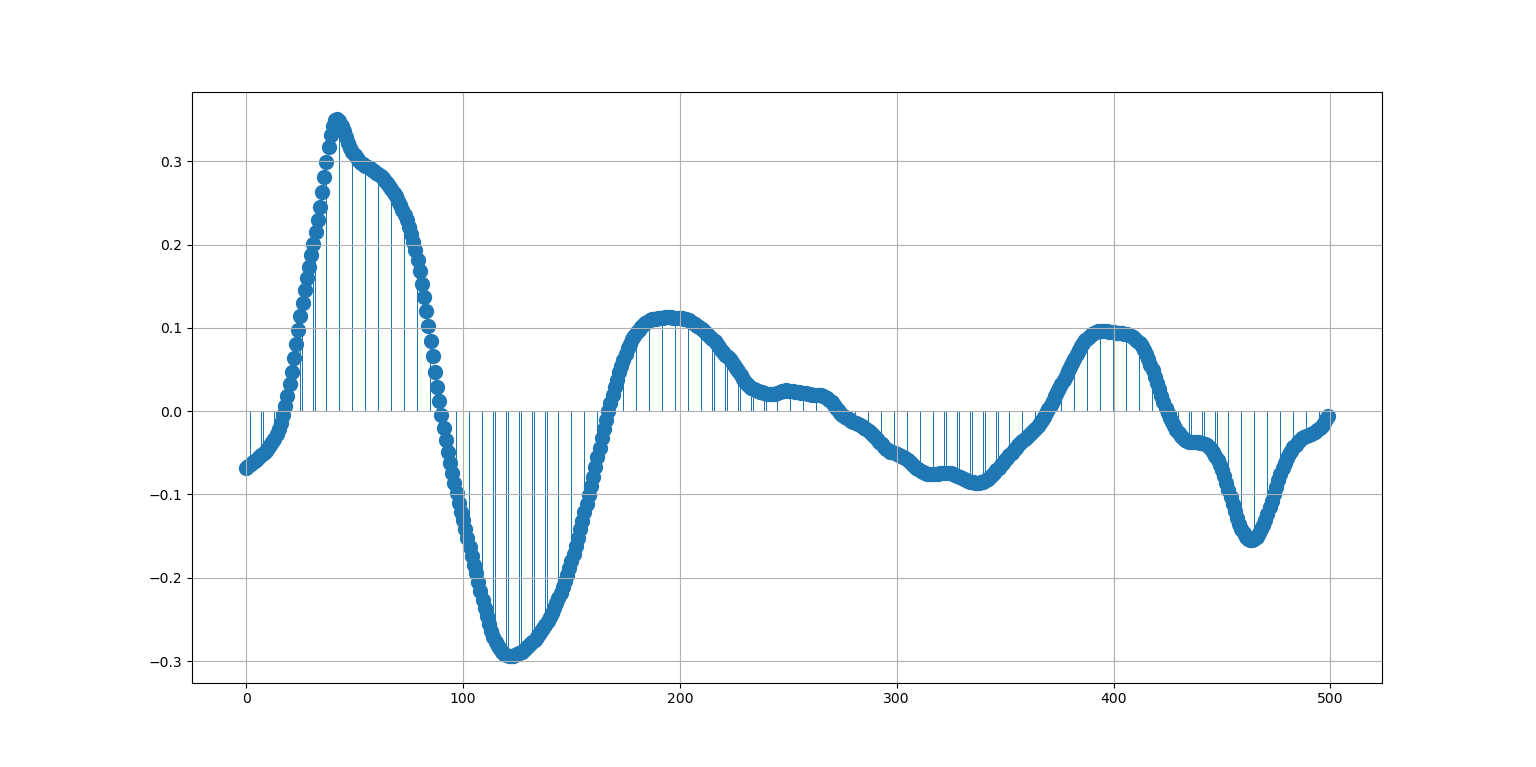
\includegraphics[width=.9\textwidth]{fig/spacend_music.png}

\begin{itemize}
	\item notion importante : le produit scalaire
	\begin{itemize}
		\item ressemblance entre deux vecteurs (signaux)
	\end{itemize}
	\item "Malédiction des grandes dimensions" :
	\begin{itemize}
		\item 44.1 kHz $\times$ 60 sec. $\times$ stereo = 5,3 millions de dim. !
	\end{itemize}
\end{itemize}
	\end{column}
    \begin{column}{0.4\textwidth}
	
	\begin{myblockred}{Produit scalaire}
	Soit 2 vecteurs $\xv$ et $\yv$ en 3D :
	\begin{align*}
	\xv &= [x_1, x_2, x_3]\\
	\yv &= [y_1, y_2, y_3]
	\end{align*}
	
	Le prod. scalaire entre $\xv$ et $\yv$ :
	\begin{align*}
		<\xv, \yv> &= x_1.y_1 + x_2.y_2 + x_3.y_3 \\
				&= \sum\limits_{i=1}^3 x_i.y_i \\
				&= ||\xv|| \ ||\yv|| \ \cos(\widehat{\xv, \yv})
	\end{align*}
	\end{myblockred}
    \end{column}
\end{columns}

\end{frame}

\begin{frame}{Quelques bases d'optimisation} %--------------------------
\begin{columns}
    \begin{column}{0.63\textwidth}
problème d'optimisation sous contraintes :
\begin{itemize}
	\item des buts sont définis
	\item des contraintes doivent être respectées
	\item le système doit trouver une solution optimale (au sens d'un critère)
\end{itemize}
	\end{column}
    \begin{column}{0.35\textwidth}
    
    \begin{figure}
    	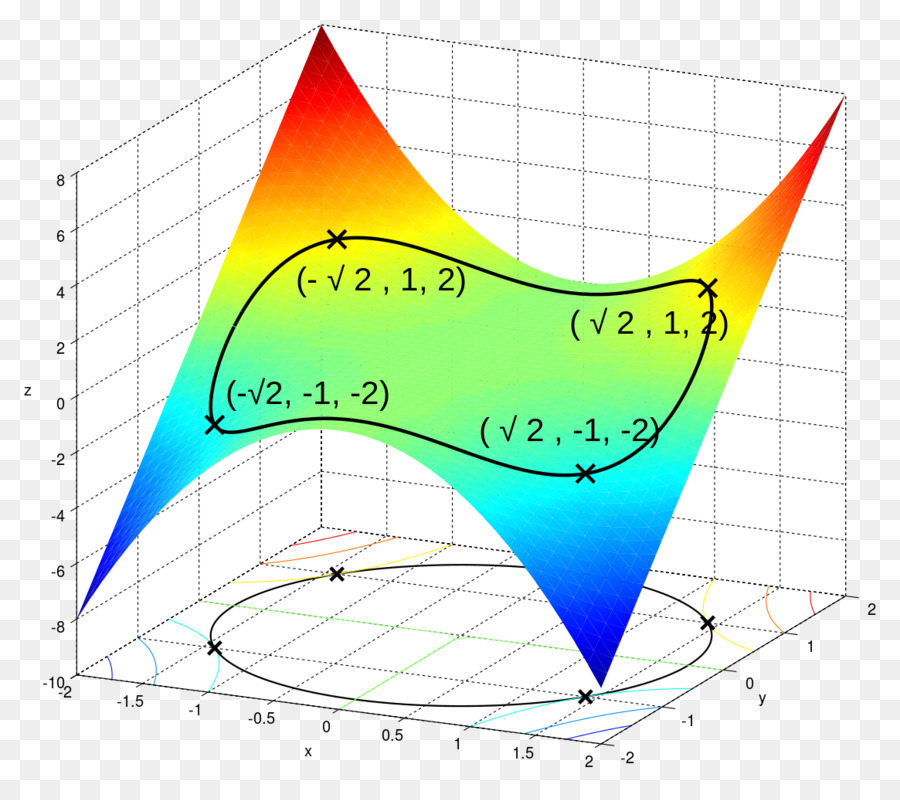
\includegraphics[width=\textwidth]{fig/lagrange_multiplier.jpg}
    	\caption{Exemple d'optimisation sous contraintes}
    \end{figure}

    \end{column}
\end{columns}

Problème sans solution optimale mais plutôt différents mix. appropriés selon le contexte (esthétique, technique) \cite{jillings_automatic_2017}

\end{frame}


\begin{frame}{Compromis exploration/exploitation} %--------------------------

\begin{figure}
	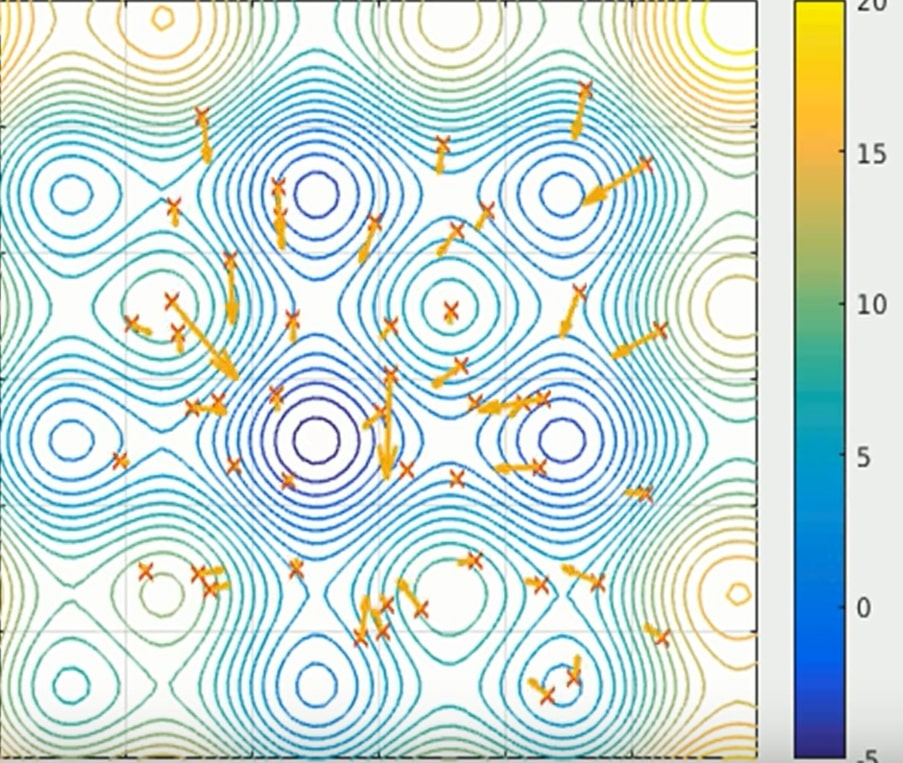
\includegraphics[width=.5\textwidth]{fig/pso_example.jpg}
	\caption{Exemple d'optimisation par essaims particulaires}
\end{figure}

voir : \url{https://youtu.be/8xycqWWqz50?t=67}
\end{frame}

\begin{frame}{Différentes méthodes d'optimisation} %--------------------------

\begin{itemize}
	\item approche des moindres carrés
	\begin{itemize}
		\item puissance de l'erreur
	\end{itemize}
	\item algorithme génétique \cite{jillings_automatic_2017}
	\begin{itemize}
		\item modélisation de la sélection naturelle
	\end{itemize}
	\item optimisation par essaims particulaires (modélisation de vol d'oiseau)
\end{itemize}
\end{frame}

%==================================================================================================
%==================================================================================================
%==================================================================================================
\section{Systèmes basés sur les données}

\begin{frame}{Systèmes basés sur les données : principe général (i)} %-----------------------------------------------------

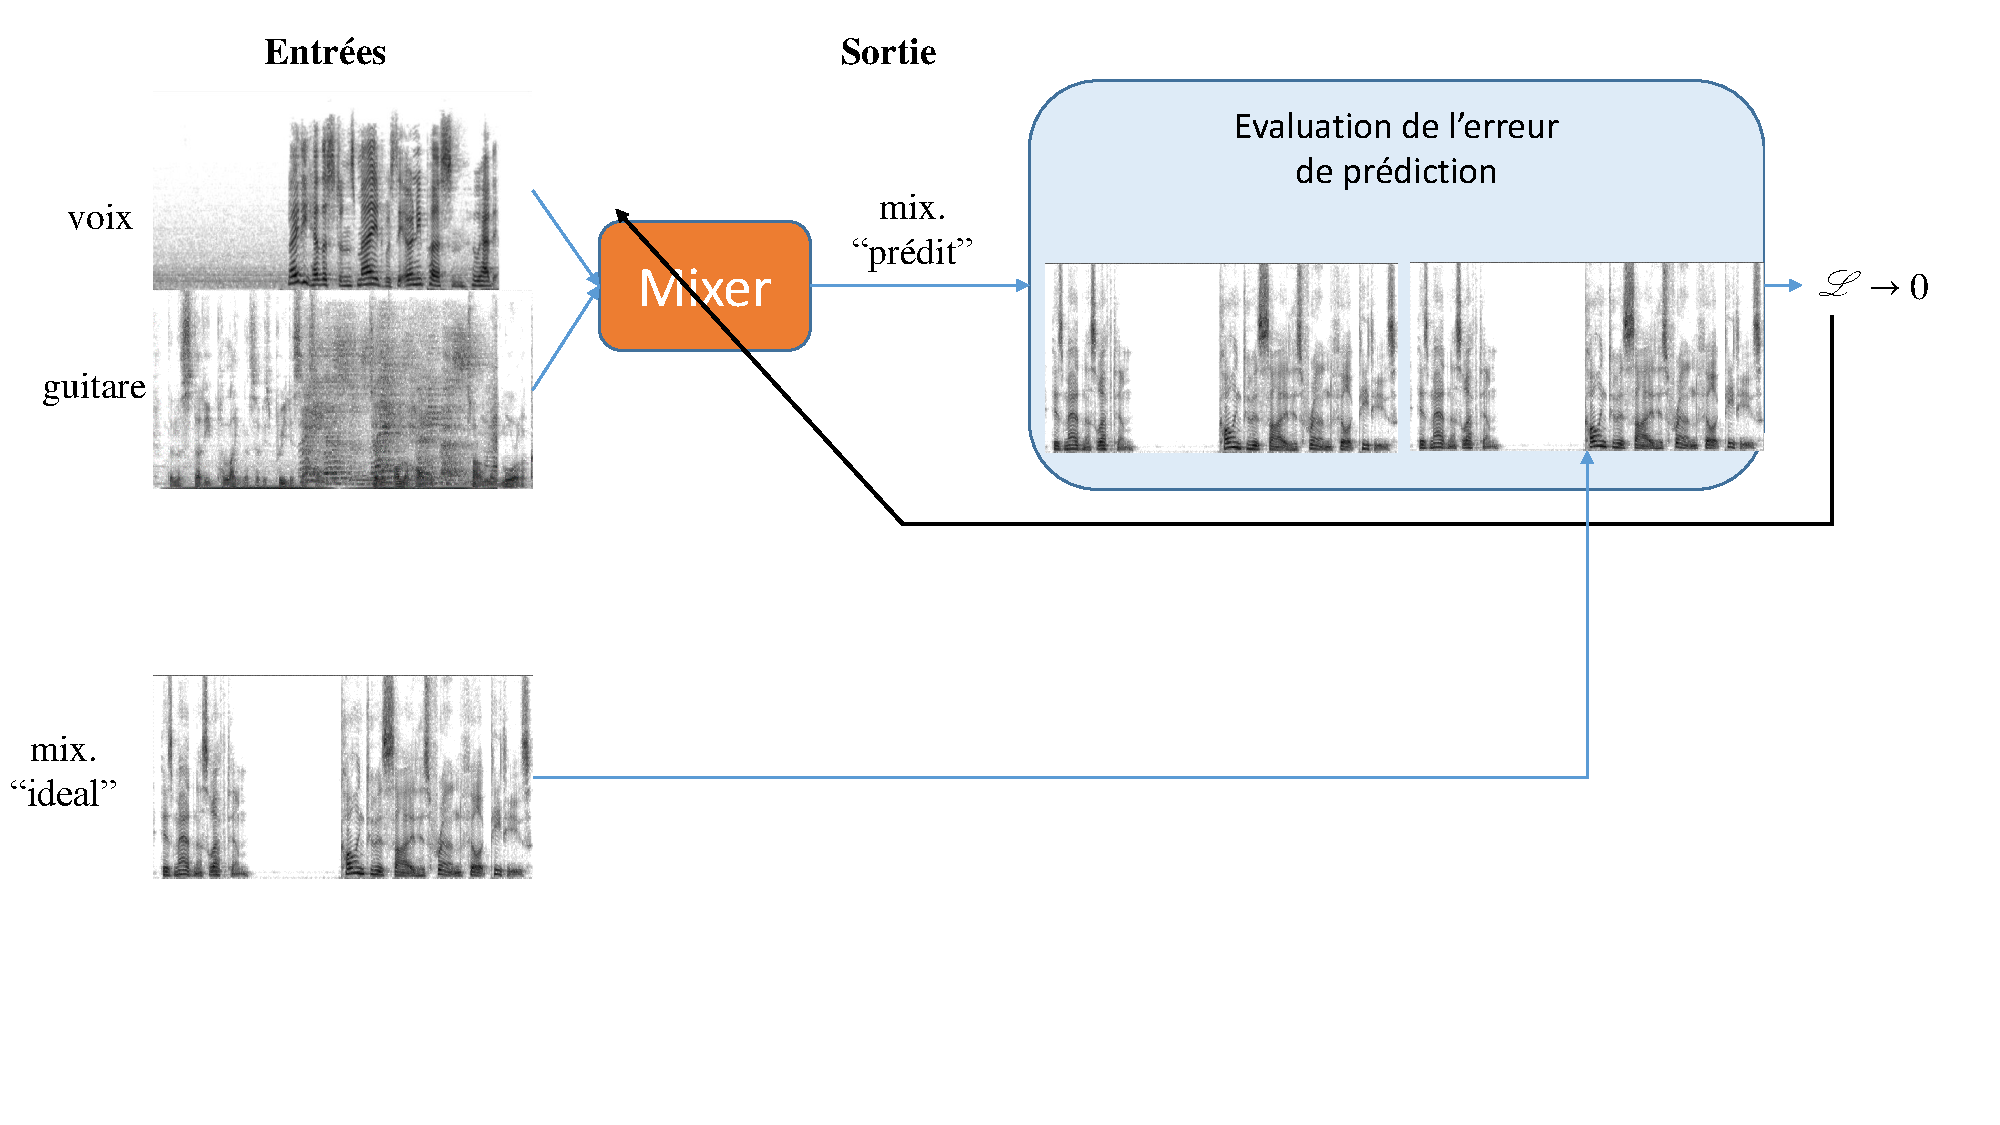
\includegraphics[width=.8\textwidth, page=1]{fig/schemas.pdf}

\end{frame}

\begin{frame}{Systèmes basés sur les données : principe général (ii)} %-----------------------------------------------------

\begin{columns}
    \begin{column}{0.6\textwidth}
\begin{itemize}
	\item Algorithme : séquence d'instructions déterministe
	\item Exemple : recette de cuisine
	\begin{itemize}
		\item mélanger 100 g. de sucre et 3 oeufs
		\item étaler, cuire...
	\end{itemize}
	\item Avec apprentissage : recette à trous
	\begin{itemize}
		\item mélanger tant d'ingrédient 1 et tant d'ingrédient 2
		\item étaler, cuire...
	\end{itemize}
	\item Processus d'apprentissage :
	\begin{itemize}
		\item essai-erreur
		\item feedback : chaud/froid
	\end{itemize}
\end{itemize}
\end{column}
    \begin{column}{0.38\textwidth}
    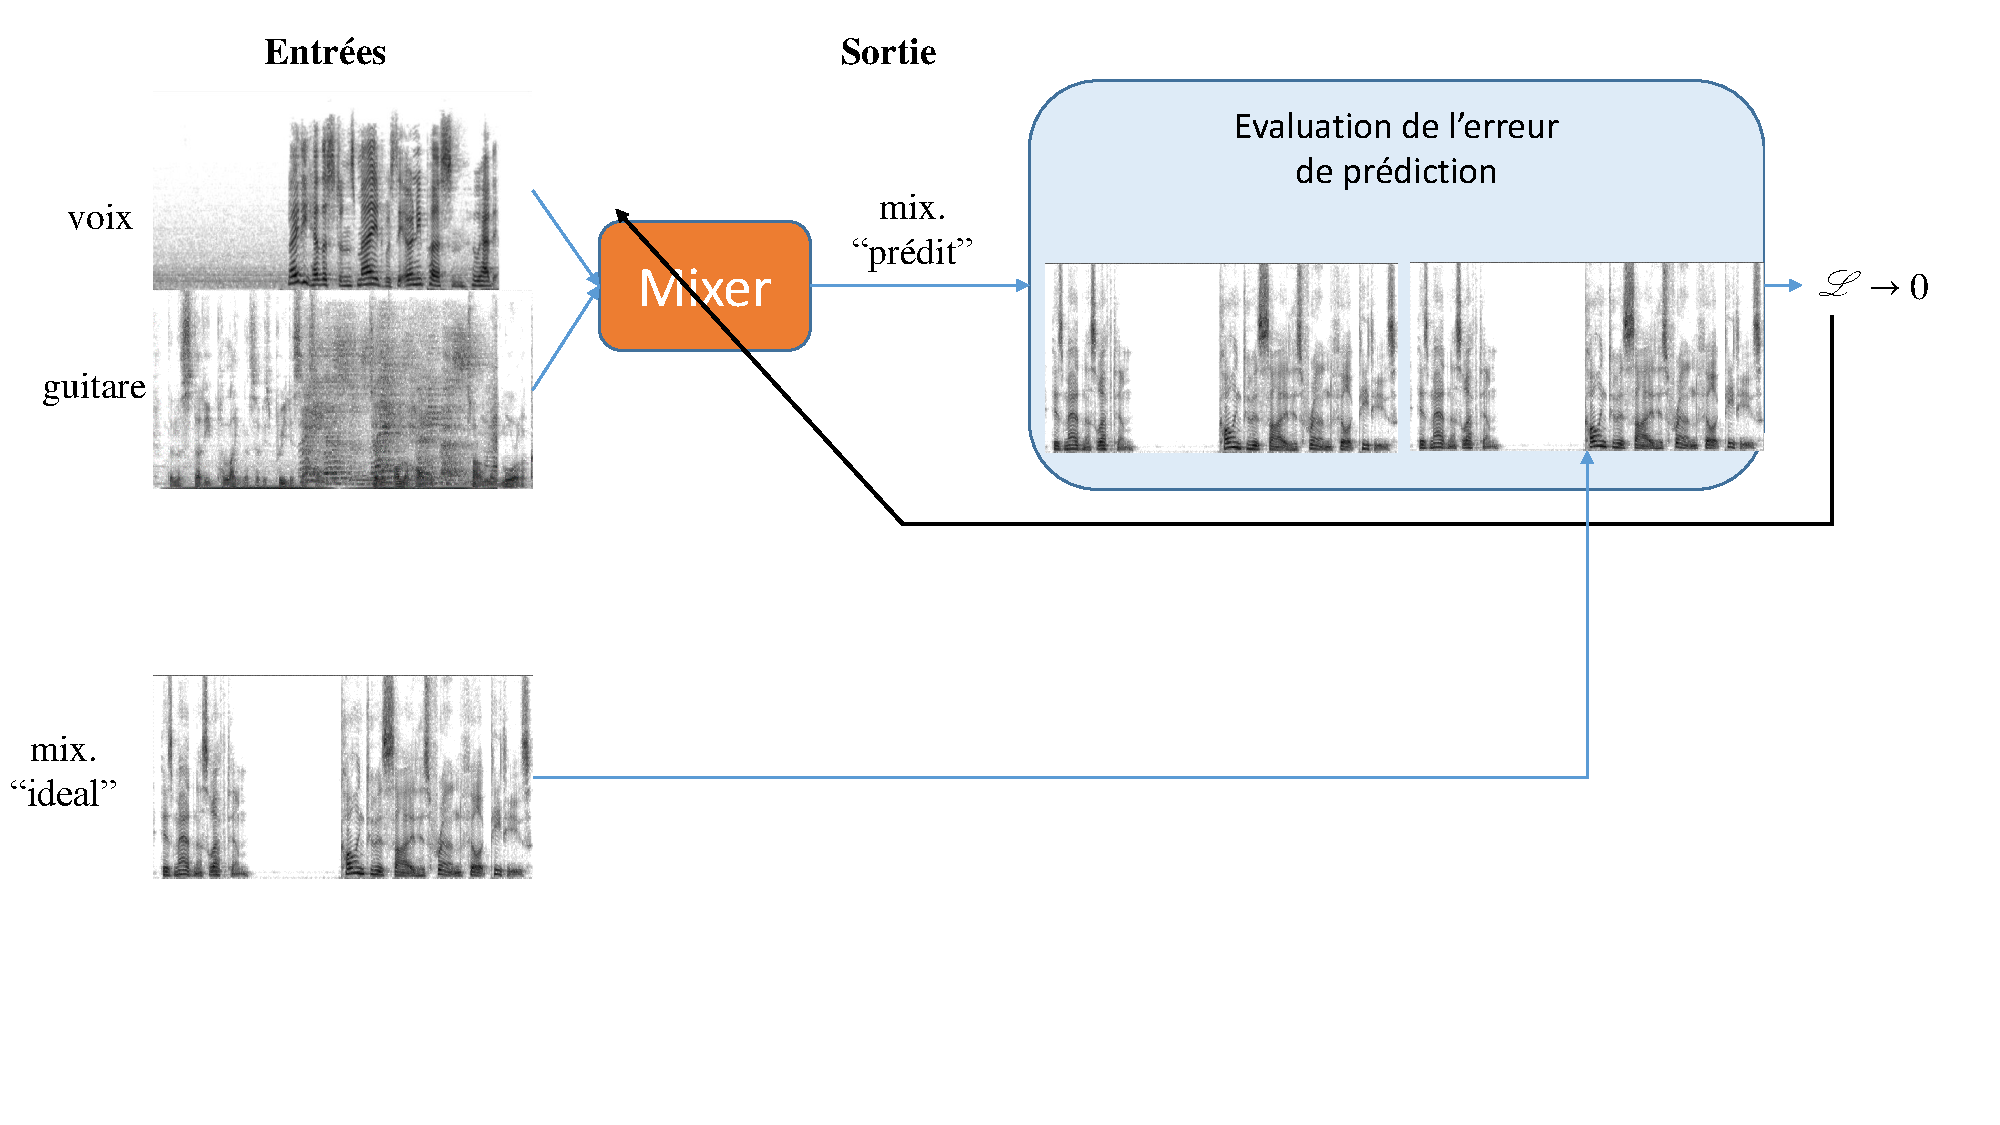
\includegraphics[width=\textwidth, page=1]{fig/schemas.pdf}
    \end{column}
\end{columns}
    
\end{frame}


\begin{frame}{Perceptron (i)} %-----------------------------------------------------

\begin{columns}
    \begin{column}{0.6\textwidth}
Modèle de neurone de grenouille (Rosenblatt, 1958) :
\begin{align*}
	y &= f(w_0 x_0 + ... + w_{n-1} x_{n-1} + b) \\
	y &= f\left( \sum\limits_{i=0}^{n-1}	 w_i x_i + b\right)
\end{align*}
analogie : "séparer" l'espace des "x" en deux

    \end{column}
    \begin{column}{0.38\textwidth}
		\begin{figure}
		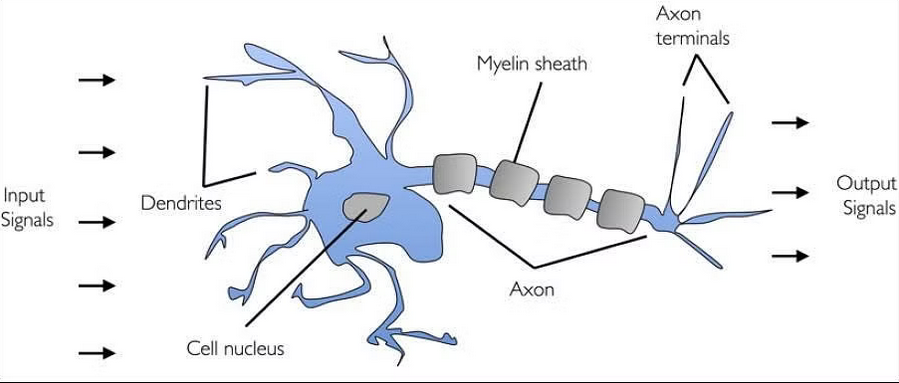
\includegraphics[width=\linewidth]{fig/biological_neuron.png}
		\caption{Illustration d'un neurone}
		\end{figure}
		\begin{figure}
		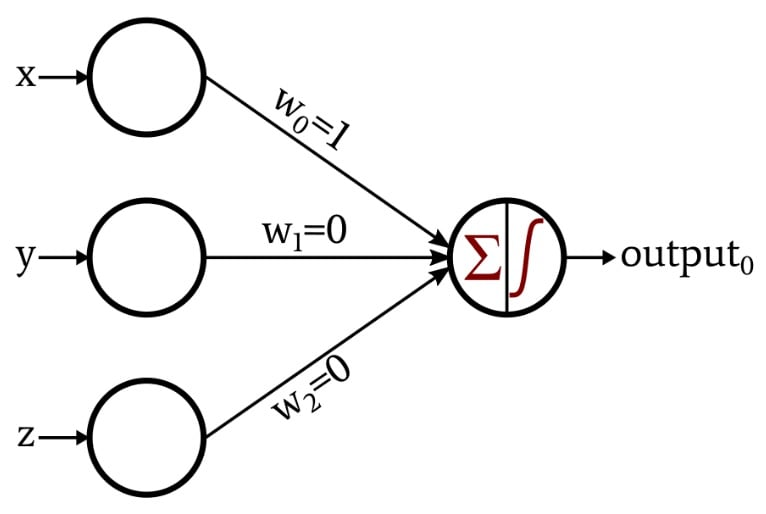
\includegraphics[width=0.55\linewidth]{fig/perceptron.jpg}
		\caption{Modèle simpliste de neurone}
		\end{figure}
    \end{column}
\end{columns}

\end{frame}

\begin{frame}{Perceptron - (ii)} %-----------------------------------------------------

\begin{columns}
    \begin{column}{0.6\textwidth}
Modèle de neurone de grenouille (Rosenblatt, 1958) :
\begin{align*}
	y &= f(w_0 x_0 + ... + w_{n-1} x_{n-1} + b) \\
	y &= f\left( \sum\limits_{i=0}^{n-1}	 w_i x_i + b\right)
\end{align*}
analogie : "séparer" l'espace des $x_i$ en deux

\vspace{1cm}
voir \url{https://deeperplayground.org}

    \end{column}
    \begin{column}{0.38\textwidth}
		\begin{figure}
		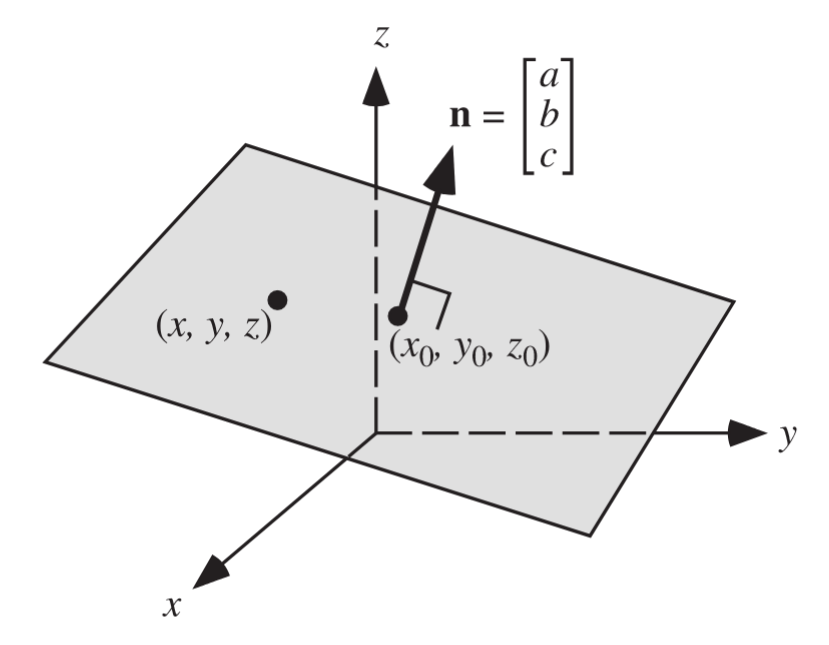
\includegraphics[width=.7\linewidth]{fig/plan.png}
		\caption{Plan défini par le vecteur $\textbf{n}$}
		\end{figure}
		\begin{figure}
		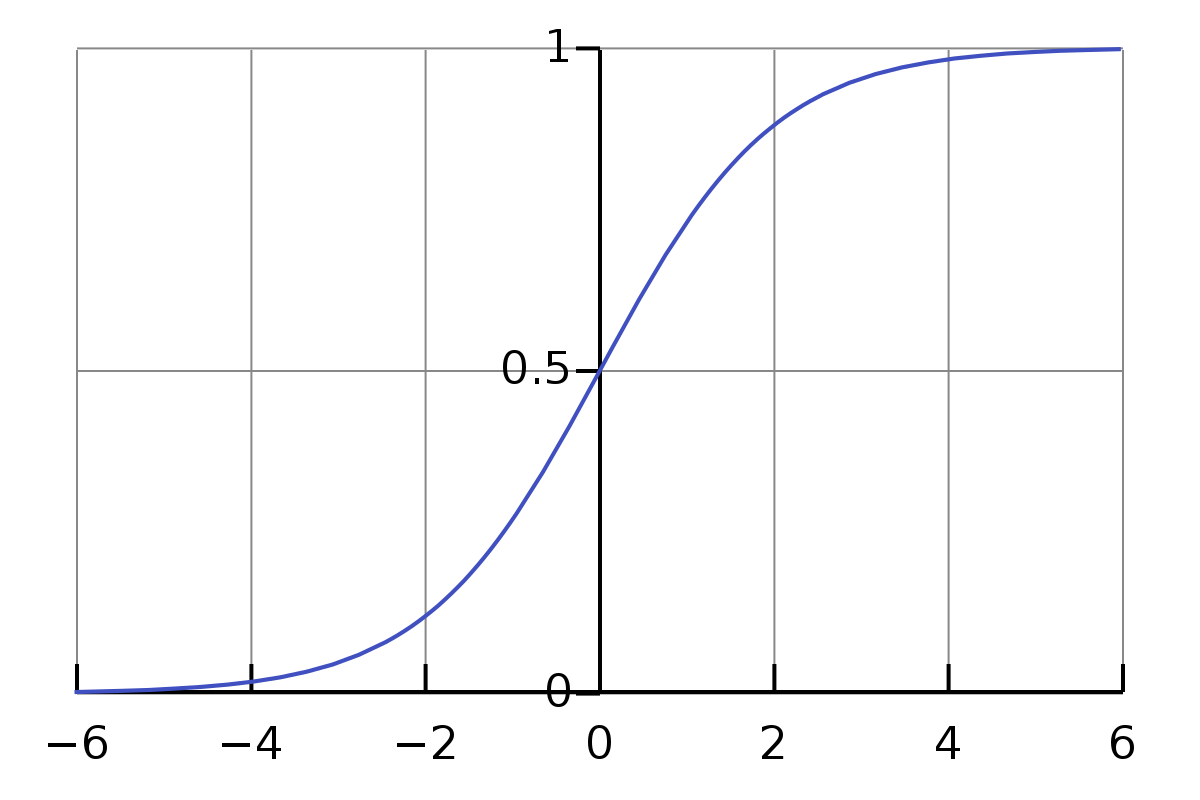
\includegraphics[width=.7\linewidth]{fig/sigmoid.png}
		\caption{Fonction d'activation sigmoïde}
		\end{figure}
    \end{column}
\end{columns}

\end{frame}


\begin{frame}{Architectures de réseau de neurones - perceptron multi-couches} %-----------------------------------------------------
\begin{columns}
    \begin{column}{0.48\textwidth}

\begin{itemize}
	\item empiler les perceptrons
	\begin{itemize}
		\item très lourd
		\item l'apprentissage ne converge pas ! 
\end{itemize}
	\item suffisant en théorie (théorème d'approximation universelle)
	\item il faut ajouter des \emph{a priori} dans le système
	\begin{itemize}
		\item exemples : dépendance dans le temps, structure harmonique...
	\end{itemize}
\end{itemize}

    \end{column}
    \begin{column}{0.48\textwidth}
    \begin{figure}
		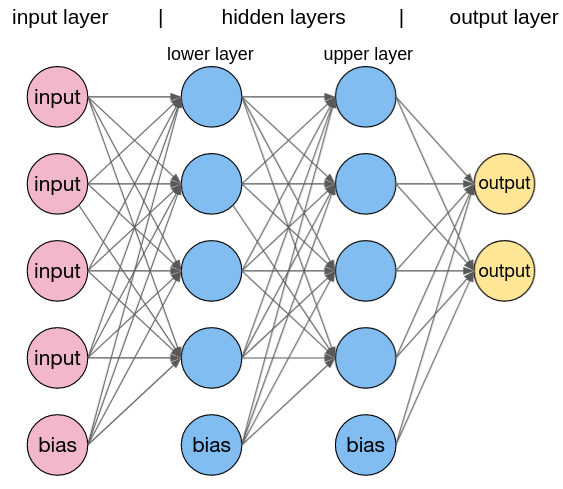
\includegraphics[width=.6\textwidth]{fig/mlp.png}
		\caption{Perceptron multi-couches}
	\end{figure}
	
    \end{column}
\end{columns}

\end{frame}


\begin{frame}{Architectures de réseau de neurones - convolutionnel} %-----------------------------------------------------
\begin{columns}
    \begin{column}{0.48\textwidth}

\begin{itemize}
	\item Réseau convolutionnel \cite{gu_recent_2018}
	\begin{itemize}
		\item léger
		\item permet de considérer le contexte "local" (ex: temps/fréquence)
	\end{itemize}
	\item hypothèse : invariance dans le temps et les fréquences
	\item exemple : recherche de contours, structures...
	
\end{itemize}

    \end{column}
    \begin{column}{0.48\textwidth}

	
    \begin{figure}
		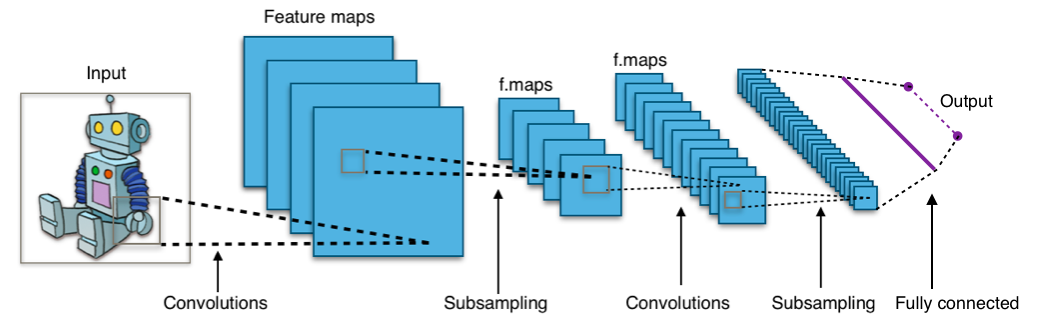
\includegraphics[width=\textwidth]{fig/cnn.png}
		\caption{Réseau convolutionnel}
	\end{figure}
	
    \end{column}
\end{columns}

\end{frame}


\begin{frame}{Architectures de réseau de neurones - récurrent} %-----------------------------------------------------
\begin{columns}
    \begin{column}{0.68\textwidth}

\begin{itemize}
	
	\item réseau de neurones récurrents
	\begin{itemize}
		\item permet de considérer le contexte à moyen terme
		\item "plus l'info est loin dans le temps, moins elle est importante"
		\item peu couteux
		\item pas évident à entrainer
	\end{itemize}
	
	\item<2-> alternativement : modèle d'"attention" \cite{lin_survey_2022}
	\begin{itemize}
		\item<2-> permet de piocher de l'information à long terme
		\item<2-> voir \url{https://www.youtube.com/watch?v=CsQNF9s78Nc}
	\end{itemize}
	\end{itemize}
	\end{column}
	\begin{column}{0.3\textwidth}
	\begin{figure}
		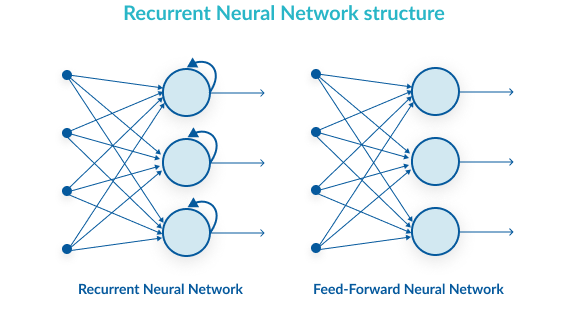
\includegraphics[width=.8\textwidth, trim=0 50 300 50, clip]{fig/rnn.png}
		\caption{Réseau récurrent}
	\end{figure}
	
    \end{column}
\end{columns}

\end{frame}



\begin{frame}{Procédure d'apprentissage} %-----------------------------------------------------

On cherche la combinaison des paramètres $\theta_0, \theta_1, ...$ qui minimise la mesure d'erreur $J(\theta_0, \theta_1, ...)$

\begin{columns}
    \begin{column}{0.48\textwidth}
Algorithme de la "descente de gradient"
	\begin{itemize}\small
		\item suivre la pente descendante de la métrique d'erreur
		\item (besoin d'un réseau de neurone "dérivable")
		\item (on rétropropage le gradient de l'erreur pour actualiser les $\theta_i$)
	\end{itemize}
En pratique, on a $\sim$10 millions de $\theta_i$ !

\only<2->{
Challenges :
\begin{itemize}
	\item trouver une mesure d'erreur $J(\theta_0, \theta_1, ...)$ pertinente ET "dérivable"
	\item avoir beaucoup de données
\end{itemize}
	}
    \end{column}
    \begin{column}{0.48\textwidth}
    \begin{figure}
		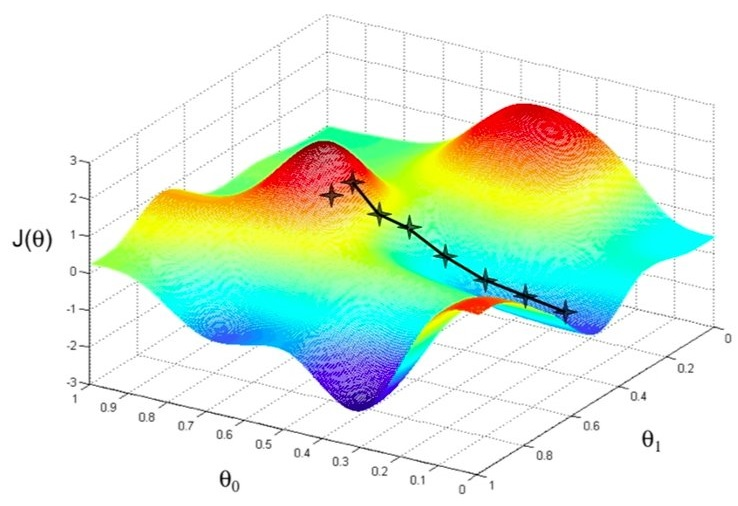
\includegraphics[width=\textwidth]{fig/gradient_descent.jpg}
		\caption{Descente de gradient}
	\end{figure}
    \end{column}
\end{columns}

\end{frame}

\begin{frame}{Console de mixage "différentiable"} %----------------

\begin{figure}
	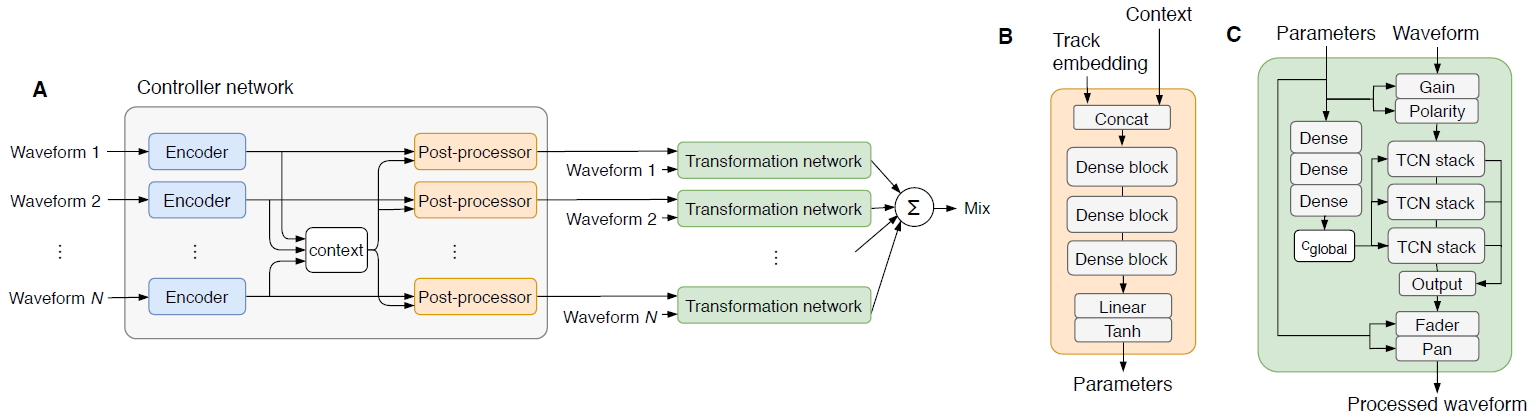
\includegraphics[width=\textwidth]{fig/steinmetz2021_diffmix.png}
	\caption{Architecture de DNN de mixage automatique de \cite{steinmetz_automatic_2020}}
\end{figure}
écouter \url{https://csteinmetz1.github.io/dmc-icassp2021/}

\begin{columns}
    \begin{column}{0.48\textwidth}
		%
    \end{column}
    \begin{column}{0.48\textwidth}
		%
    \end{column}
\end{columns}
\end{frame}

\begin{frame}{} %-----------------------------------------------------

\begin{figure}
	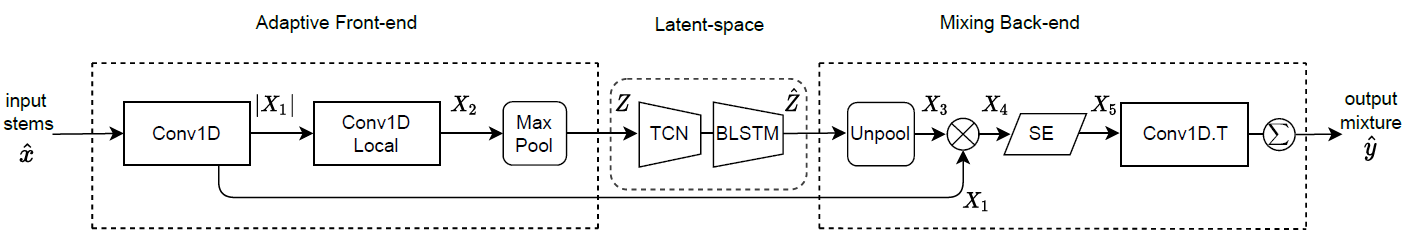
\includegraphics[width=\textwidth]{fig/martinez_ramirez2022_architecture.png}
	\caption{Architecture de DNN de mixage automatique de \cite{martinez-ramirez_automatic_2022}}
\end{figure}
écouter \url{https://marco-martinez-sony.github.io/FxNorm-automix/AUDIO_SAMPLES.html}

\begin{columns}
    \begin{column}{0.48\textwidth}
		%
    \end{column}
    \begin{column}{0.48\textwidth}
		%
    \end{column}
\end{columns}
\end{frame}


\begin{frame}{Base de données} %---------------------------------

	\begin{itemize}
		\item peu de données de session multi-pistes et mixage pro associé
		\begin{itemize}
			\item ENST-Drums : 3h de batterie (8 pistes)
			\item MedleyDB : 196 chansons, $\sim$7h \cite{bittner_medleydb_2014}
		\end{itemize}
		\item réemploi d'autres base de données (séparation de sources musicales)
		\begin{itemize}
			\item MUSDB18 (voir \cite{martinez-ramirez_automatic_2022})
		\end{itemize}
		\item représentation inégales des instruments \cite{bittner_medleydb_2014}
		\begin{itemize}
			\item voix plus présente que la clarinette basse
		\end{itemize}
	\end{itemize}

\end{frame}

%==================================================================================================
%==================================================================================================
%==================================================================================================
\section{Interface humain-machine}
\begin{frame}{Différents niveaux d'interactions} %-----------------------------------------------------
\begin{columns}
    \begin{column}{0.48\textwidth}
		Différentes applications :
		\begin{itemize}
			\item aide à la décision/préprocessing vs. full automatic (personne devant la console)
			\item amateur vs. pro
		\end{itemize}

    \end{column}
    \begin{column}{0.48\textwidth}
		Différents niveaux d'interaction :
		\begin{itemize}
			\item Automatique
			\item Indépendant
			\item Recommandation
			\item Découverte (exploration)
		\end{itemize}
    \end{column}
\end{columns}
\end{frame}

\begin{frame}{Automatique} %-----------------------------------------------------
\begin{columns}
    \begin{column}{0.48\textwidth}
		\begin{itemize}
			\item production amateur
			\item petit concert
			\item mix. étalon
			\item jeu vidéo \cite{schmidt_interactive_2003}
		\end{itemize}
    \end{column}
    \begin{column}{0.48\textwidth}
		%
    \end{column}
\end{columns}
\end{frame}

\begin{frame}{Indépendant} %-----------------------------------------------------
\begin{columns}

    \begin{column}{0.48\textwidth}
	    Supervisé par un.e opérateurice
		\begin{itemize}
			\item réduction de diaphonie (repisse micro)
			\item synchronisation entre micro (couple + appoints)
			\item Démasquage fréquentiel \cite{wichern_comparison_2015}
			\item pour amateur et pro.
		\end{itemize}
    \end{column}
    \begin{column}{0.48\textwidth}
		\begin{figure}
			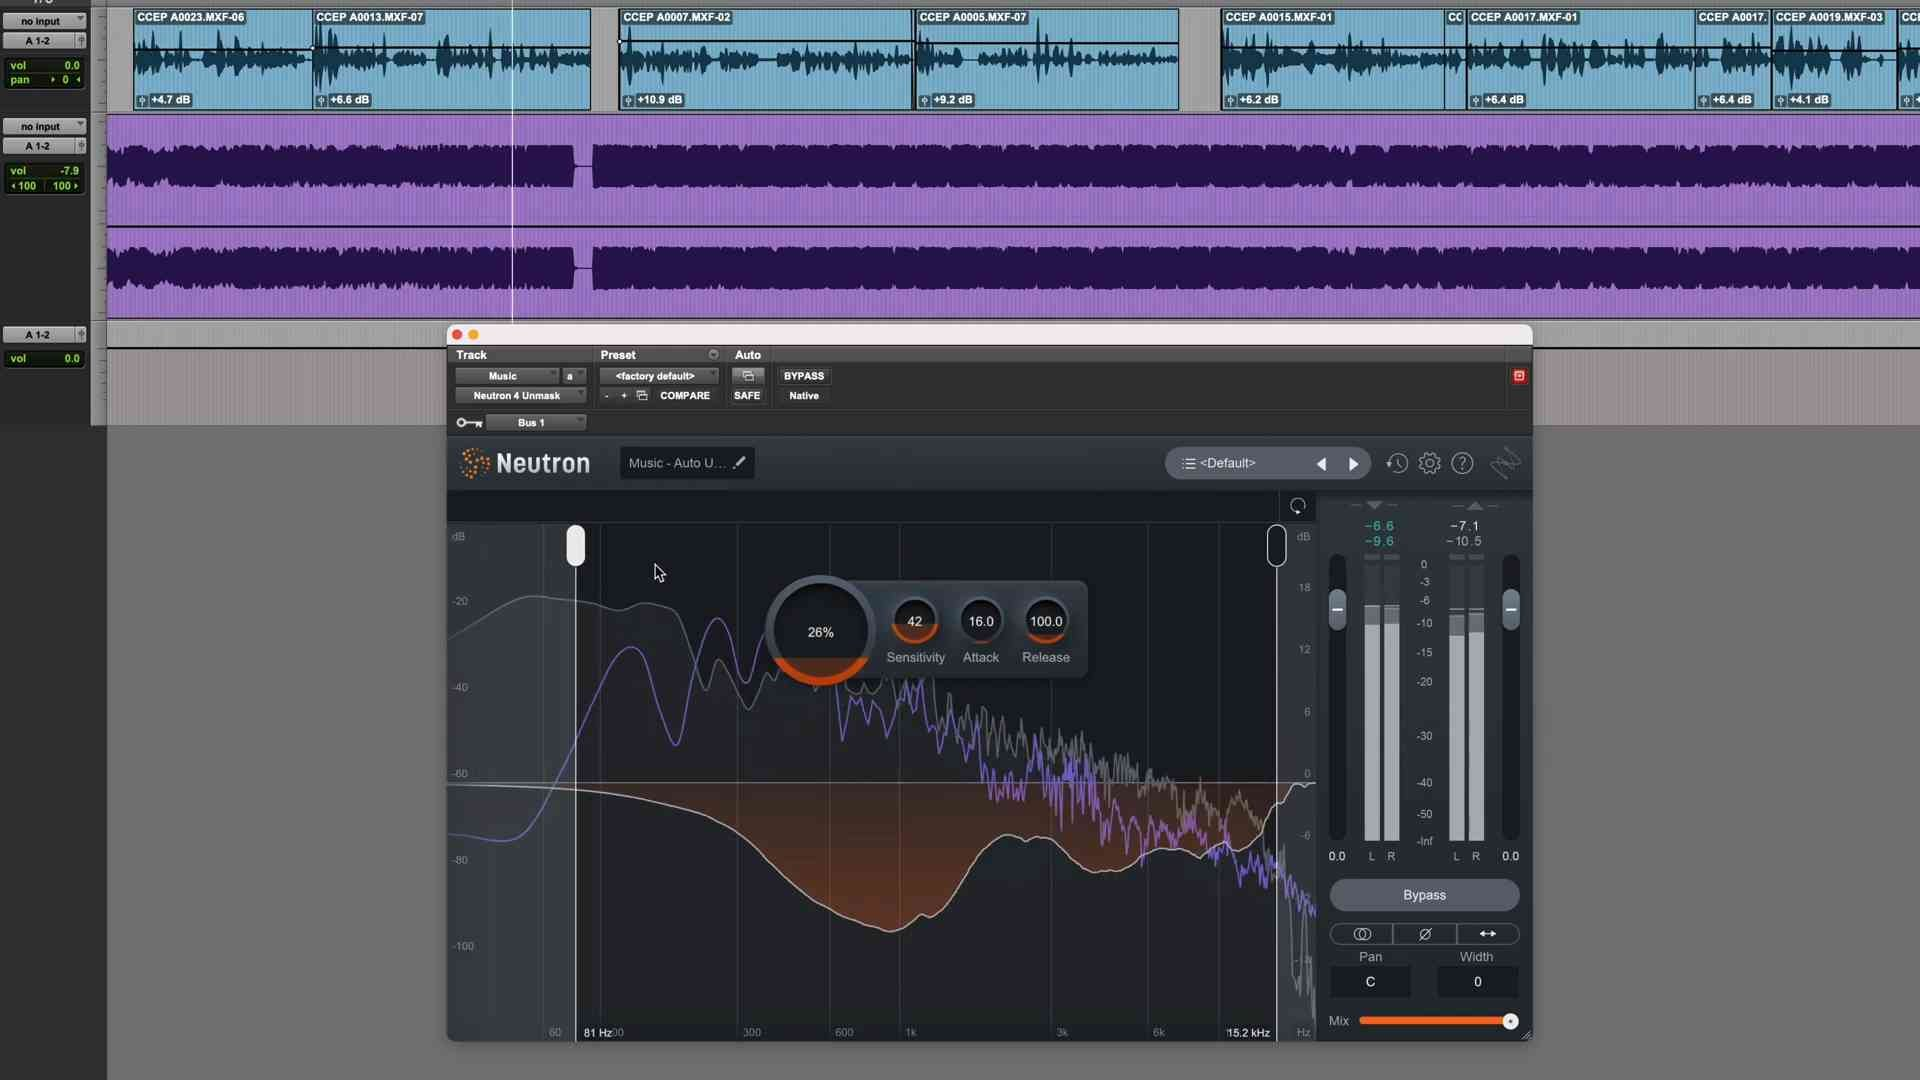
\includegraphics[width=\textwidth]{fig/neutron_unmask.jpg}
			\caption{Izotope Neutron, démasque auto.}
		\end{figure}
    \end{column}
\end{columns}
Analogue aux manœuvres automatiques pour la voiture autonome
\end{frame}

\begin{frame}{Recommandation} %-----------------------------------------------------

\begin{columns}
    \begin{column}{0.48\textwidth}
	    Suggestion de traitements
		\begin{itemize}
			\item annotation automatique d'instrument
			\item annotation automatique de structure de morceau \cite{hargreaves_structural_2012}
			\item suggestion de chaine d'effets \cite{sauer_recommending_2013}
			\item suggestion de paramètres d'effets
			\item organisation des \emph{stems}
		\end{itemize}
    \end{column}
    \begin{column}{0.48\textwidth}
		\begin{figure}
			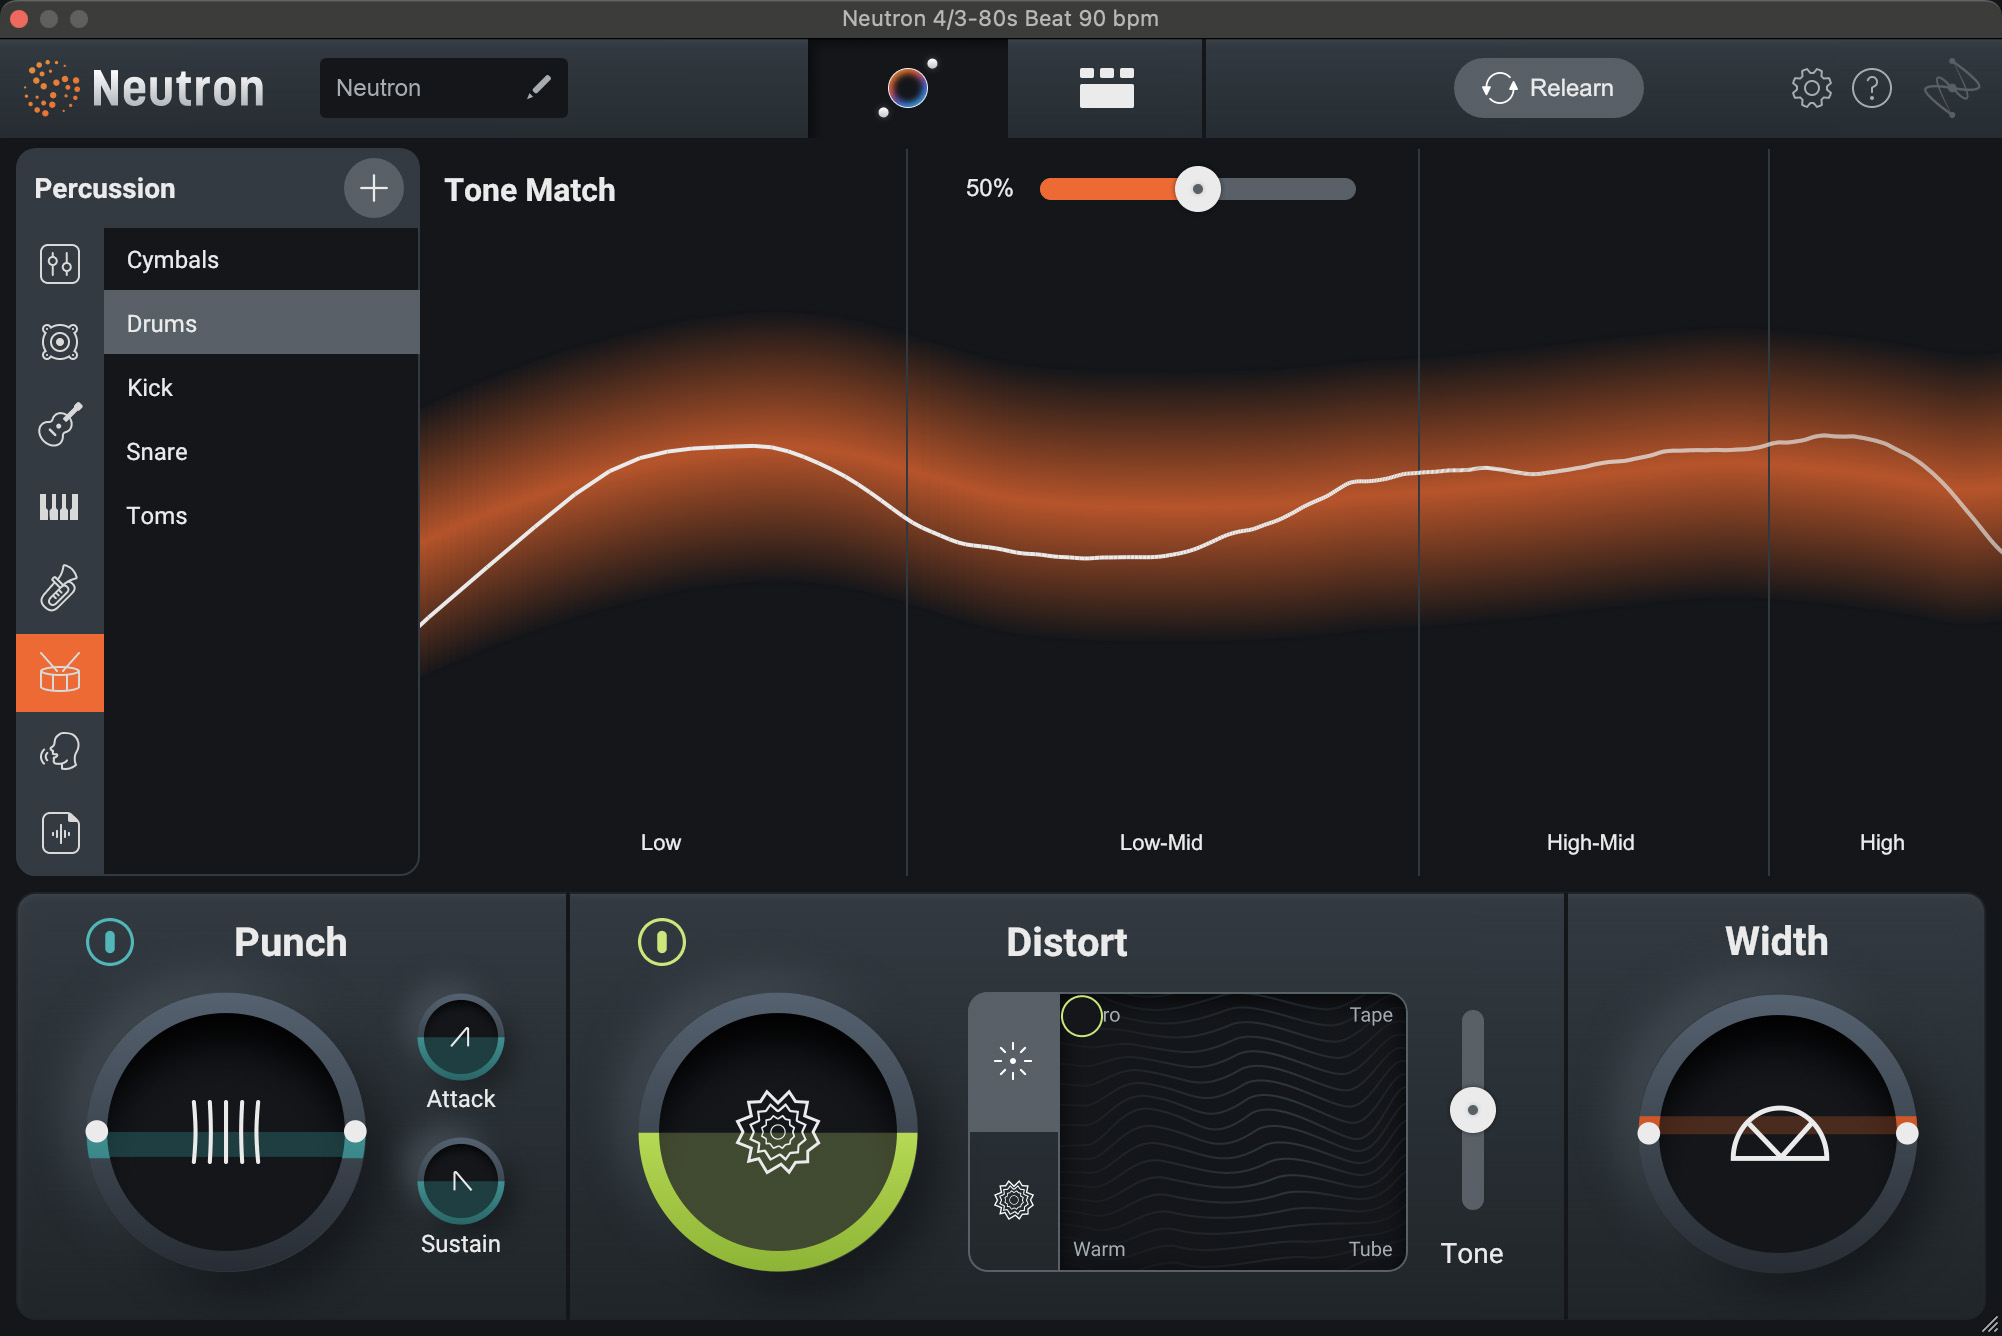
\includegraphics[width=\textwidth]{fig/neutron_spectrum_suggestion.jpg}
			\caption{Izotope Neutron, tone matching}
		\end{figure}
    \end{column}
\end{columns}
Descripteurs vers paramètres d'effets audio (voir "prompt to picture")

Avantage : interprétable et adaptable
\end{frame}

\begin{frame}{Découverte (exploration)} %----------------------------------------------

\begin{columns}
    \begin{column}{0.48\textwidth}
	    Outils d'analyse du mix
		\begin{itemize}
			\item visualisation de mix. \cite{ford_mixviz_2015}
			\item comparaison avec un mix. de référence
			\item description qualitative (textuelle) du mix.
			\item description quantitative (numérique) du mix.
			\item analyse du niveau de reverb. et de son impact sur chaque piste dans le mix. \cite{de_man_perceptual_2017}
		\end{itemize}
    \end{column}
    \begin{column}{0.48\textwidth}
		%
    \end{column}
\end{columns}

\end{frame}

%==================================================================================================
%==================================================================================================
%==================================================================================================
\section{Conclusion}

\begin{frame}{Résumé} %-----------------------------------------------------
\begin{columns}
    \begin{column}{0.58\textwidth}
    
\begin{itemize}
	\item 15 ans de recherche (depuis 2007)
	\item essor du deep learning depuis 5 ans (depuis 2016)
	\item un problème fondamentalement mal posé ?
	\begin{itemize}
		\item pas de "vérité terrain" \cite{birtchnell_automating_2018}
	\end{itemize}
\end{itemize}

\end{column}
    \begin{column}{0.42\textwidth}
    \begin{figure}
    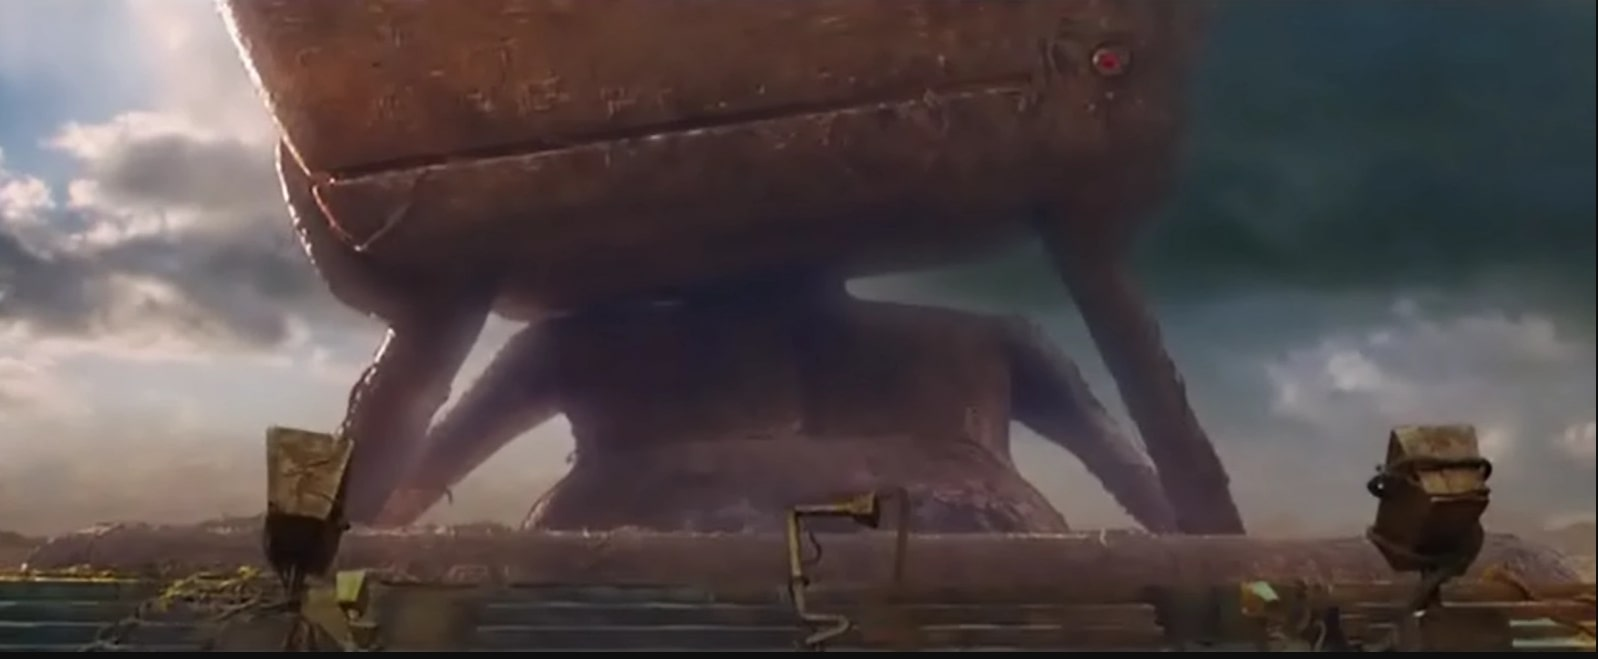
\includegraphics[width=\textwidth]{fig/deep_thought.jpg}
    \caption{"42" - H2G2}    
    \end{figure}

    \end{column}
\end{columns}
\end{frame}

\begin{frame}{Perspectives} %-----------------------------------------------------
\begin{columns}
    \begin{column}{0.58\textwidth}
		\begin{itemize}
	\item aller vers le mix. 5.1, orienté-objet...
	\item considérer différentes esthétiques de mix.
	\item vers une meilleure connaissance de l'essence de la musique
	\item réduire les tâches laborieuses en montage
		\begin{itemize}
			\item suggestion de sonothèque
			\item bruitage de pas, de "présence"
			\item nettoyage parole (bruit de bouche, etc.)
		\end{itemize}
	\item recommandation d'arrangement musical
	\begin{itemize}
		\item instrument complémentaire pour enrichir le timbre
	\end{itemize}
	\item jeu vidéo et réalité augmentée
	\begin{itemize}
		\item mixage ajouté au son local !
	\end{itemize}
\end{itemize}
    \end{column}
    \begin{column}{0.4\textwidth}
		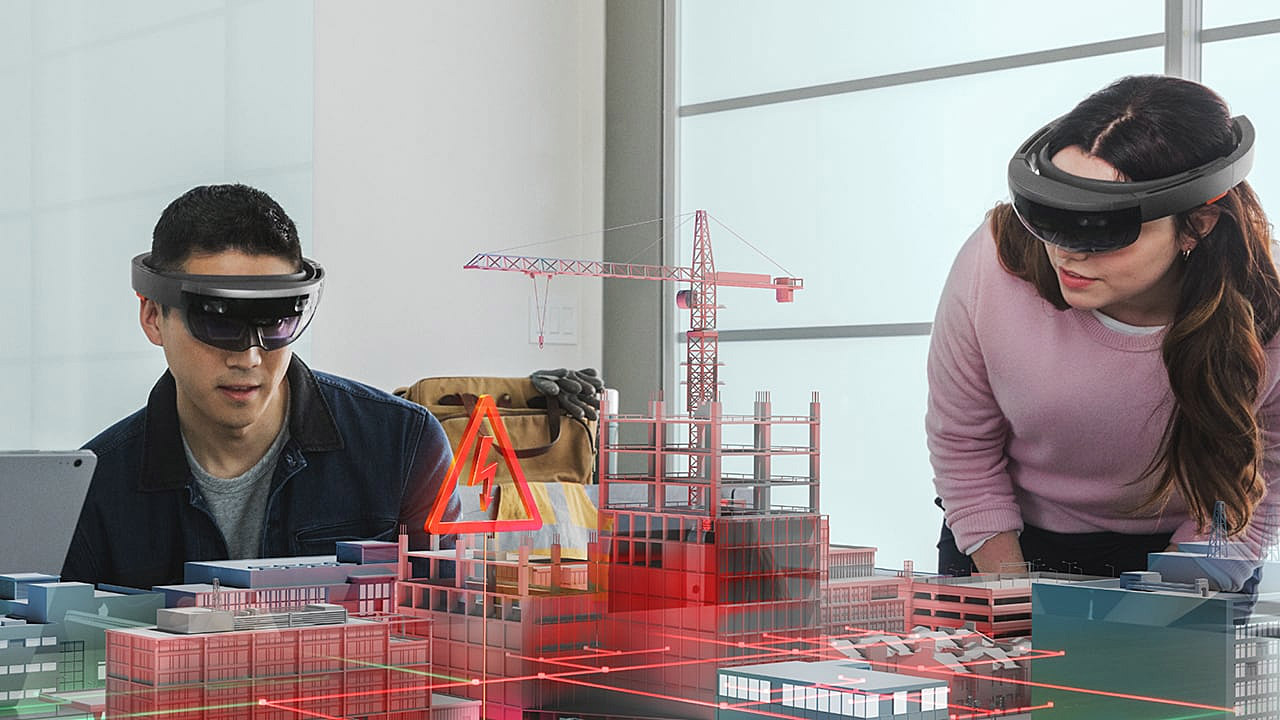
\includegraphics[width=\textwidth]{fig/microsoft-hololens-ar.jpg}
    \end{column}
\end{columns}
\end{frame}

%==================================================================================================
%==================================================================================================
%======================================== BIBLE ===================================================	
\appendix
\begin{withoutheadline}
\begin{frame}[allowframebreaks]{Bibliographie}
	\fontsize{5pt}{5pt}\selectfont
	\bibliographystyle{apalike}
	\bibliography{bible}
\end{frame}
\end{withoutheadline}

%==================================================================================================
%==================================================================================================
%======================================= TEMPLATE =================================================

%\begin{frame}{} %-----------------------------------------------------
%\end{frame}
%
%\begin{frame}{} %-----------------------------------------------------
%\begin{columns}
%    \begin{column}{0.48\textwidth}
%		%
%    \end{column}
%    \begin{column}{0.48\textwidth}
%		%
%    \end{column}
%\end{columns}
%\end{frame}

\end{document}